\documentclass[../main.tex]{subfiles}
\begin{document}

\ifSubfilesClassLoaded{
	\mainmatter
	\setcounter{chapter}{6}
}{}

\section{Drell-Yan Cross Section Ratio}
\subsection{Mass fit results}
The two datasets are analyzed separately, and a fit to the mass spectrum is performed separately for each
dataset and each target independently.
The fits to the mass distributions for Run 2-3 data are shown in \cref{fig:massfit_integrated}, and the
data is very well described by the fitting procedure outlined in \cref{M-sec:massfit_procedure}.
Similarly, the mass distributions for Run 5-6 are also shown in \cref{fig:massfit_integrated}.
\begin{figure}[htpb!]
	\begin{subfigure}{0.48\linewidth}
		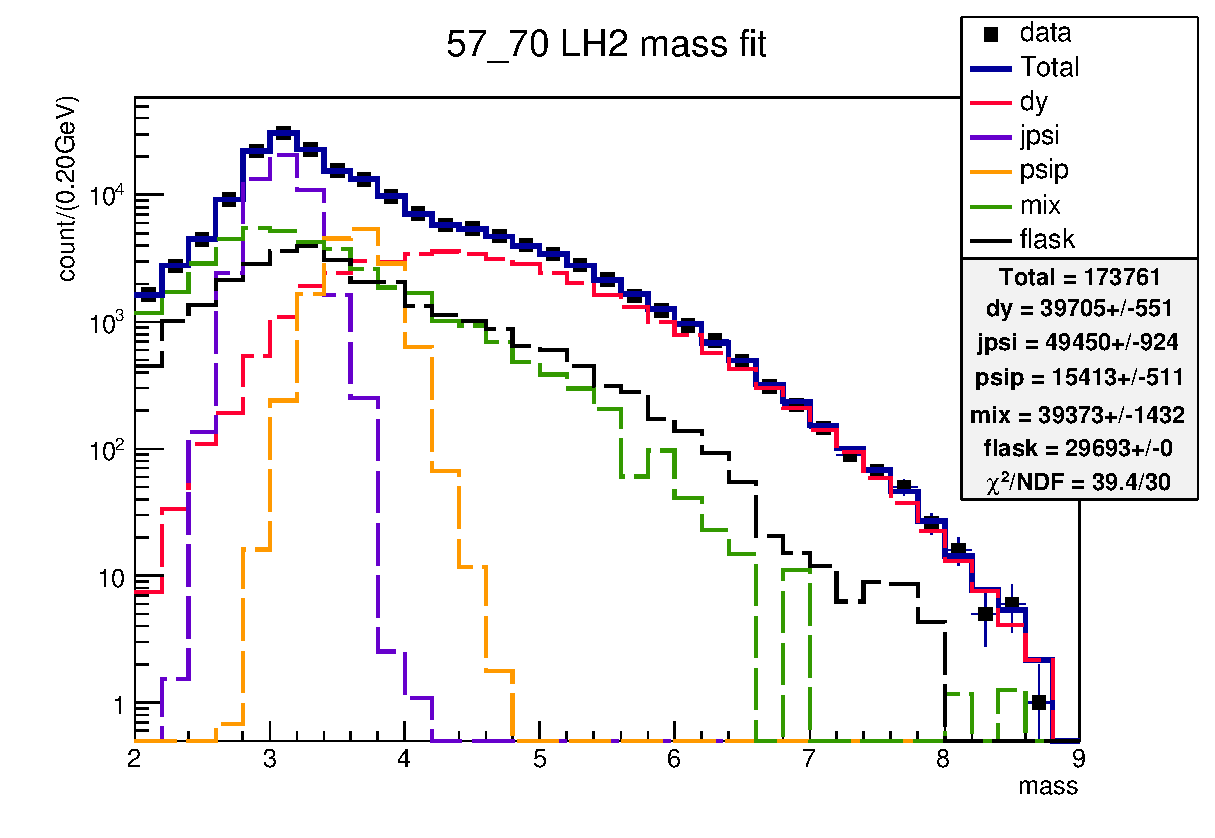
\includegraphics[width=\linewidth]{massfit/run2-3/57_70_LH2_log}
	\end{subfigure}
	\begin{subfigure}{0.48\linewidth}
		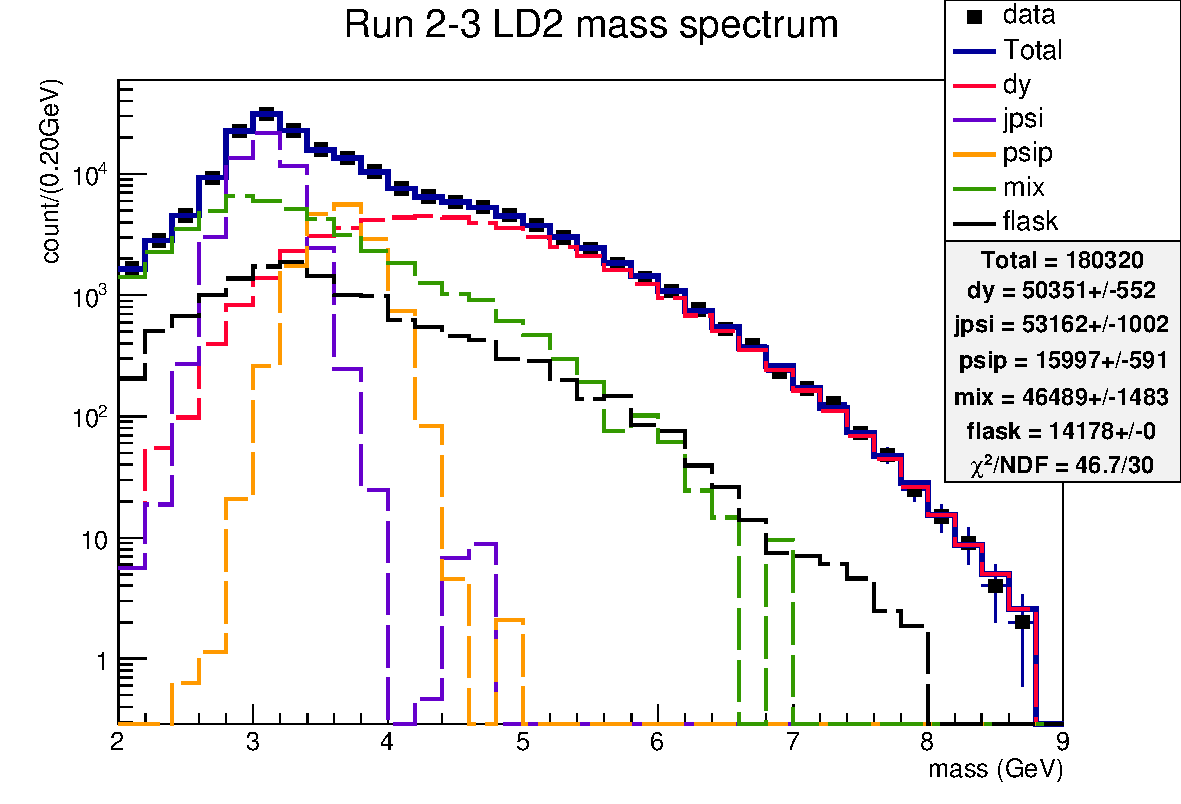
\includegraphics[width=\linewidth]{massfit/run2-3/57_70_LD2_log}
	\end{subfigure}
	\\
	\begin{subfigure}{0.48\linewidth}
		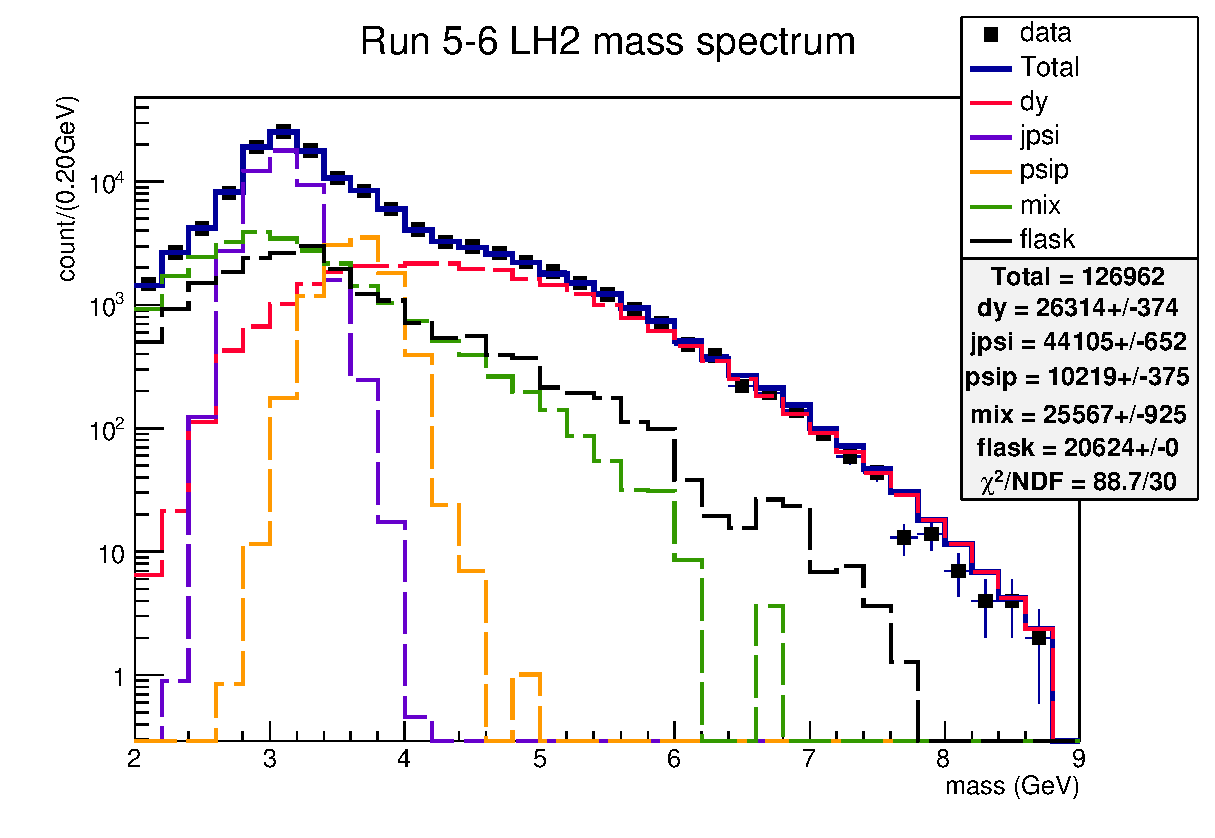
\includegraphics[width=\linewidth]{massfit/run5-6/5_6_LH2_log}
	\end{subfigure}
	\begin{subfigure}{0.48\linewidth}
		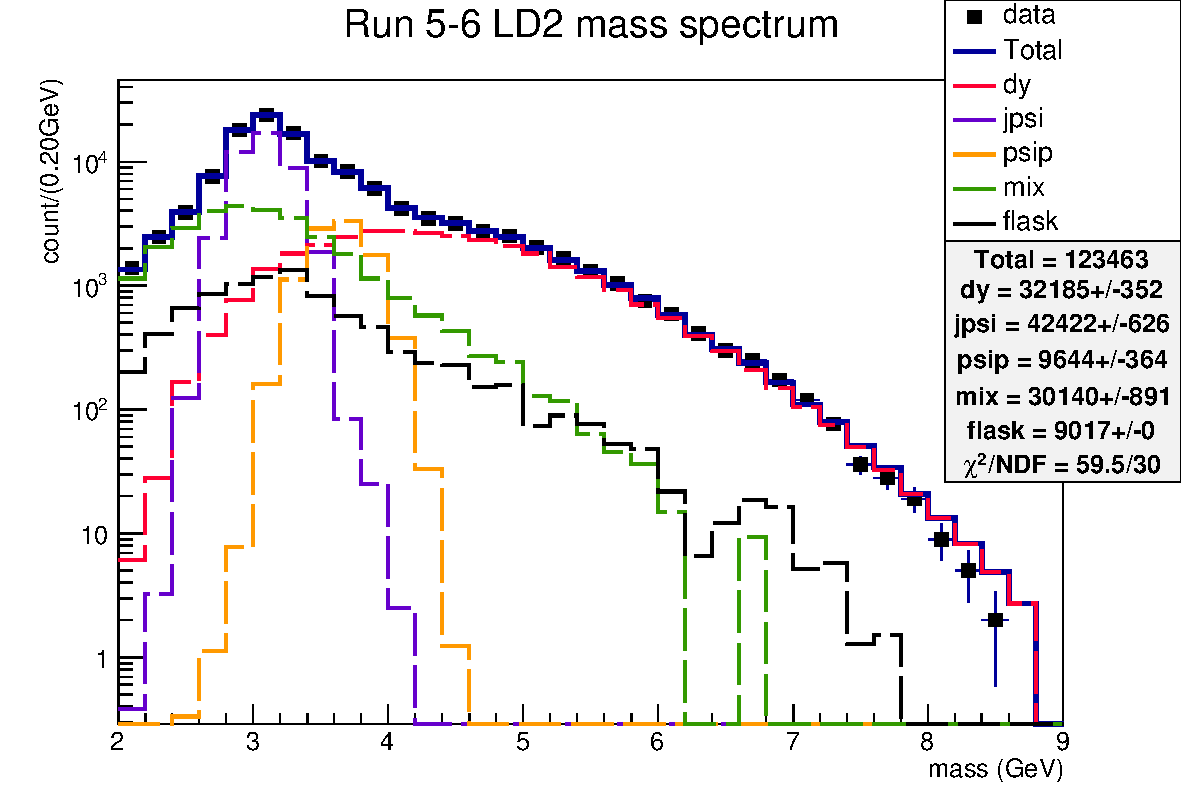
\includegraphics[width=\linewidth]{massfit/run5-6/5_6_LD2_log}
	\end{subfigure}
	\caption{The mass spectrum for \ce{LH_2}(left) and \ce{LD_2}(right) targets data for Run 2-3 (top) and Run 5-6 (bottom).}
	\label{fig:massfit_integrated}
\end{figure}
With the yields for different processes obtained from the mass fits, 
the cross section ratio as a function of $x_T$ can be calculated following \cref{M-subsec:contamination},
and are shown in \cref{fig:CSR_MF_xT} and tabulated in \cref{tab:DY-MF-x2}.
\begin{figure}[htpb!]
	\centering
	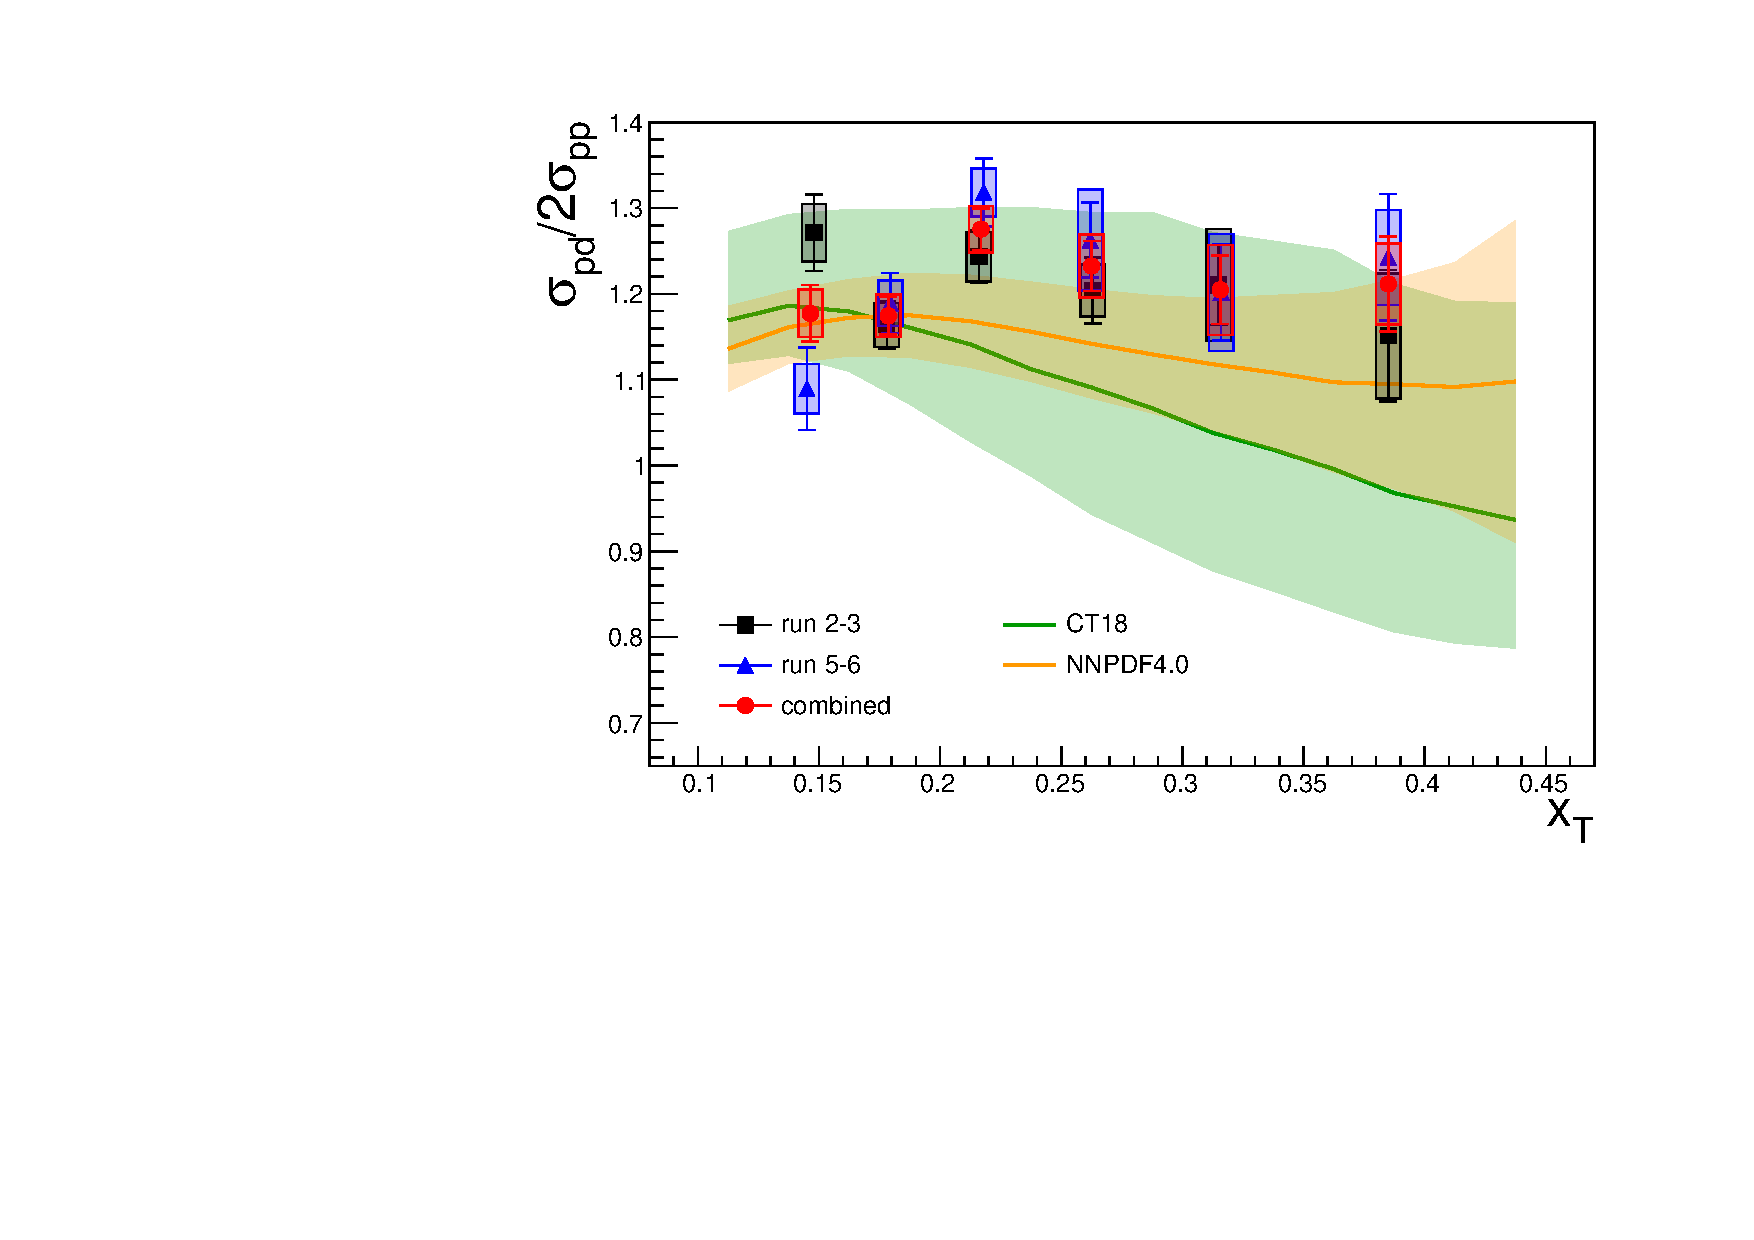
\includegraphics[width=0.7\linewidth]{DY-csr/MF_full_xT_syst}
	\caption{The extracted Drell-Yan cross section ratio as a function of $x_T$
		using the mass fit method from Run 2-3 (black squares) and Run 5-6 (blue triangles),
		as well as the combined result (red circles). The curve corresponds to calculations
		using CT18 (green) and NNPDF4.0 (orange).}
	\label{fig:CSR_MF_xT}
\end{figure}
\begin{table}[htpb!]
	\centering
	\caption{The extracted Drell-Yan cross section ratios as a function of $x_T$ using the mass fit method.}
	\label{tab:DY-MF-x2}
	\begin{tabular}{c|ccc}
\hline
$x_T$ bin    & Run 2-3                 & Run 5-6                 & Combined                \\ \hline
$0.13-0.16$  & $1.271\pm0.045\pm0.034$ & $1.090\pm0.048\pm0.029$ & $1.177\pm0.033\pm0.028$ \\
$0.16-0.195$ & $1.164\pm0.028\pm0.026$ & $1.189\pm0.035\pm0.027$ & $1.174\pm0.022\pm0.025$ \\
$0.195-0.24$ & $1.243\pm0.031\pm0.029$ & $1.318\pm0.039\pm0.028$ & $1.275\pm0.024\pm0.027$ \\
$0.24-0.29$  & $1.204\pm0.038\pm0.030$ & $1.263\pm0.044\pm0.059$ & $1.232\pm0.029\pm0.037$ \\
$0.29-0.35$  & $1.210\pm0.047\pm0.065$ & $1.202\pm0.056\pm0.068$ & $1.205\pm0.040\pm0.052$ \\
$0.35-0.45$  & $1.151\pm0.077\pm0.073$ & $1.243\pm0.074\pm0.055$ & $1.212\pm0.055\pm0.047$ \\ \hline
\end{tabular}

\end{table}

The extracted cross section ratio from the two datasets are consistent with each other within uncertainties.
The red points in \cref{fig:CSR_MF_xT} represent results from the combined analysis following the procedure in \cref{M-subsec:combine}.
\FloatBarrier

\subsubsection{Effect of the updated target contamination correction}
\label{subsubsec:contamination_result}
As discussed in \cref{M-subsec:contamination}, incorrect target contamination corrections were used
in previous publications and the effect is shown in \cref{fig:contaimination_CSR}.
The overall effect is a roughly \SI{2}{\percent} shift in the ratio. 
This correction only affects the results from Run~2-3 as the later runs utilize commercial pure deuterium.
The updated corrections are used throughout this thesis.
\begin{figure}[htpb!]
	\centering
	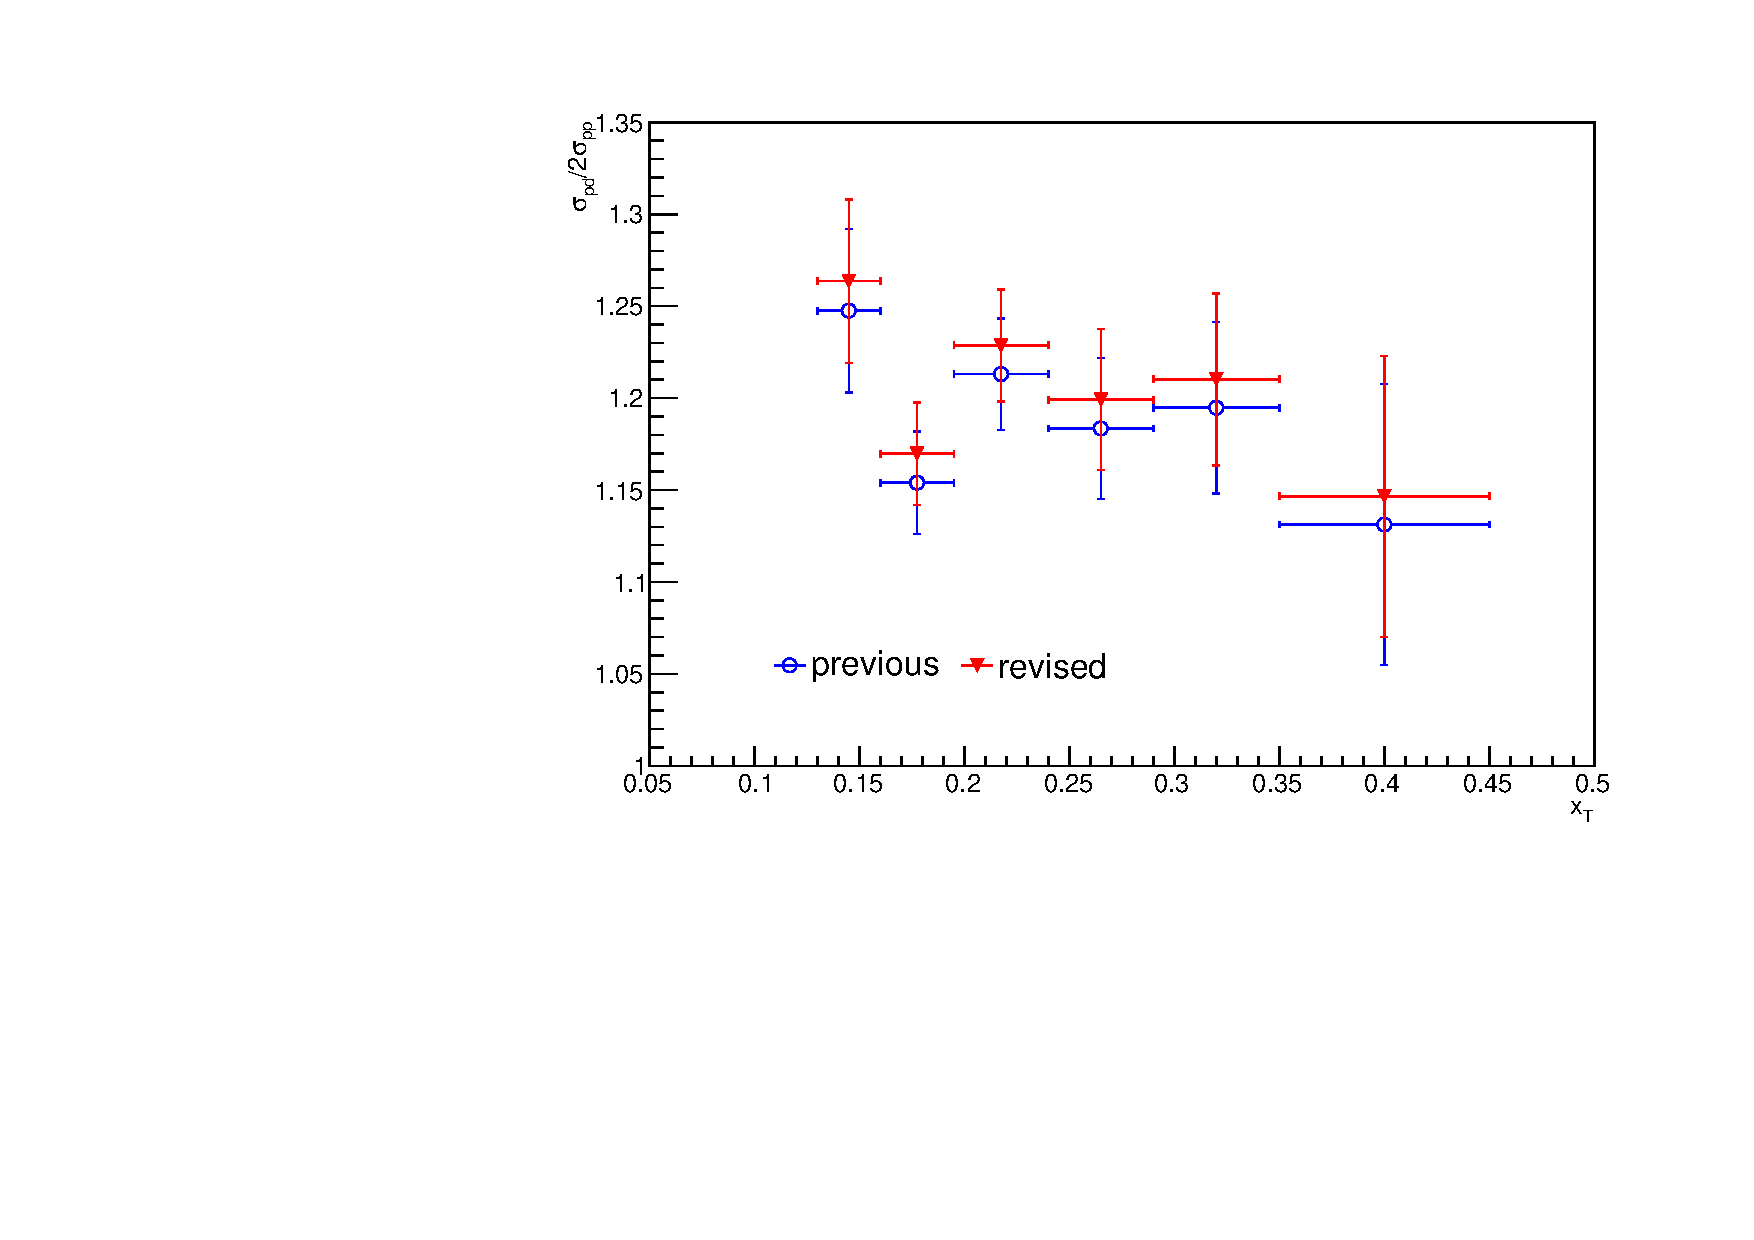
\includegraphics[width=0.6\linewidth]{DY-csr/Compare_targetCorr}
	\caption{The effect of the updated target contamination correction on the Drell-Yan
		cross section. The extracted cross section ratio using the revised target contamination
		is shown as red solid triangles, and the previous published version is shown as blue open
		circles. The overall effect is a roughly \SI{2}{\percent} shift in the ratio. }
	\label{fig:contaimination_CSR}
\end{figure}
\FloatBarrier

\subsubsection{Cross section ratio vs other variables}
Following a similar procedure, the Drell-Yan cross section ratios as a function of $x_B$ (\cref{fig:CSR_MF_xB})
and $x_F$ (\cref{fig:CSR_MF_xF}) are also extracted, and tabulated in \cref{tab:DY-MF-x1} and \cref{tab:DY-IE-xF} respectively.
\begin{figure}[htpb!]
	\centering
	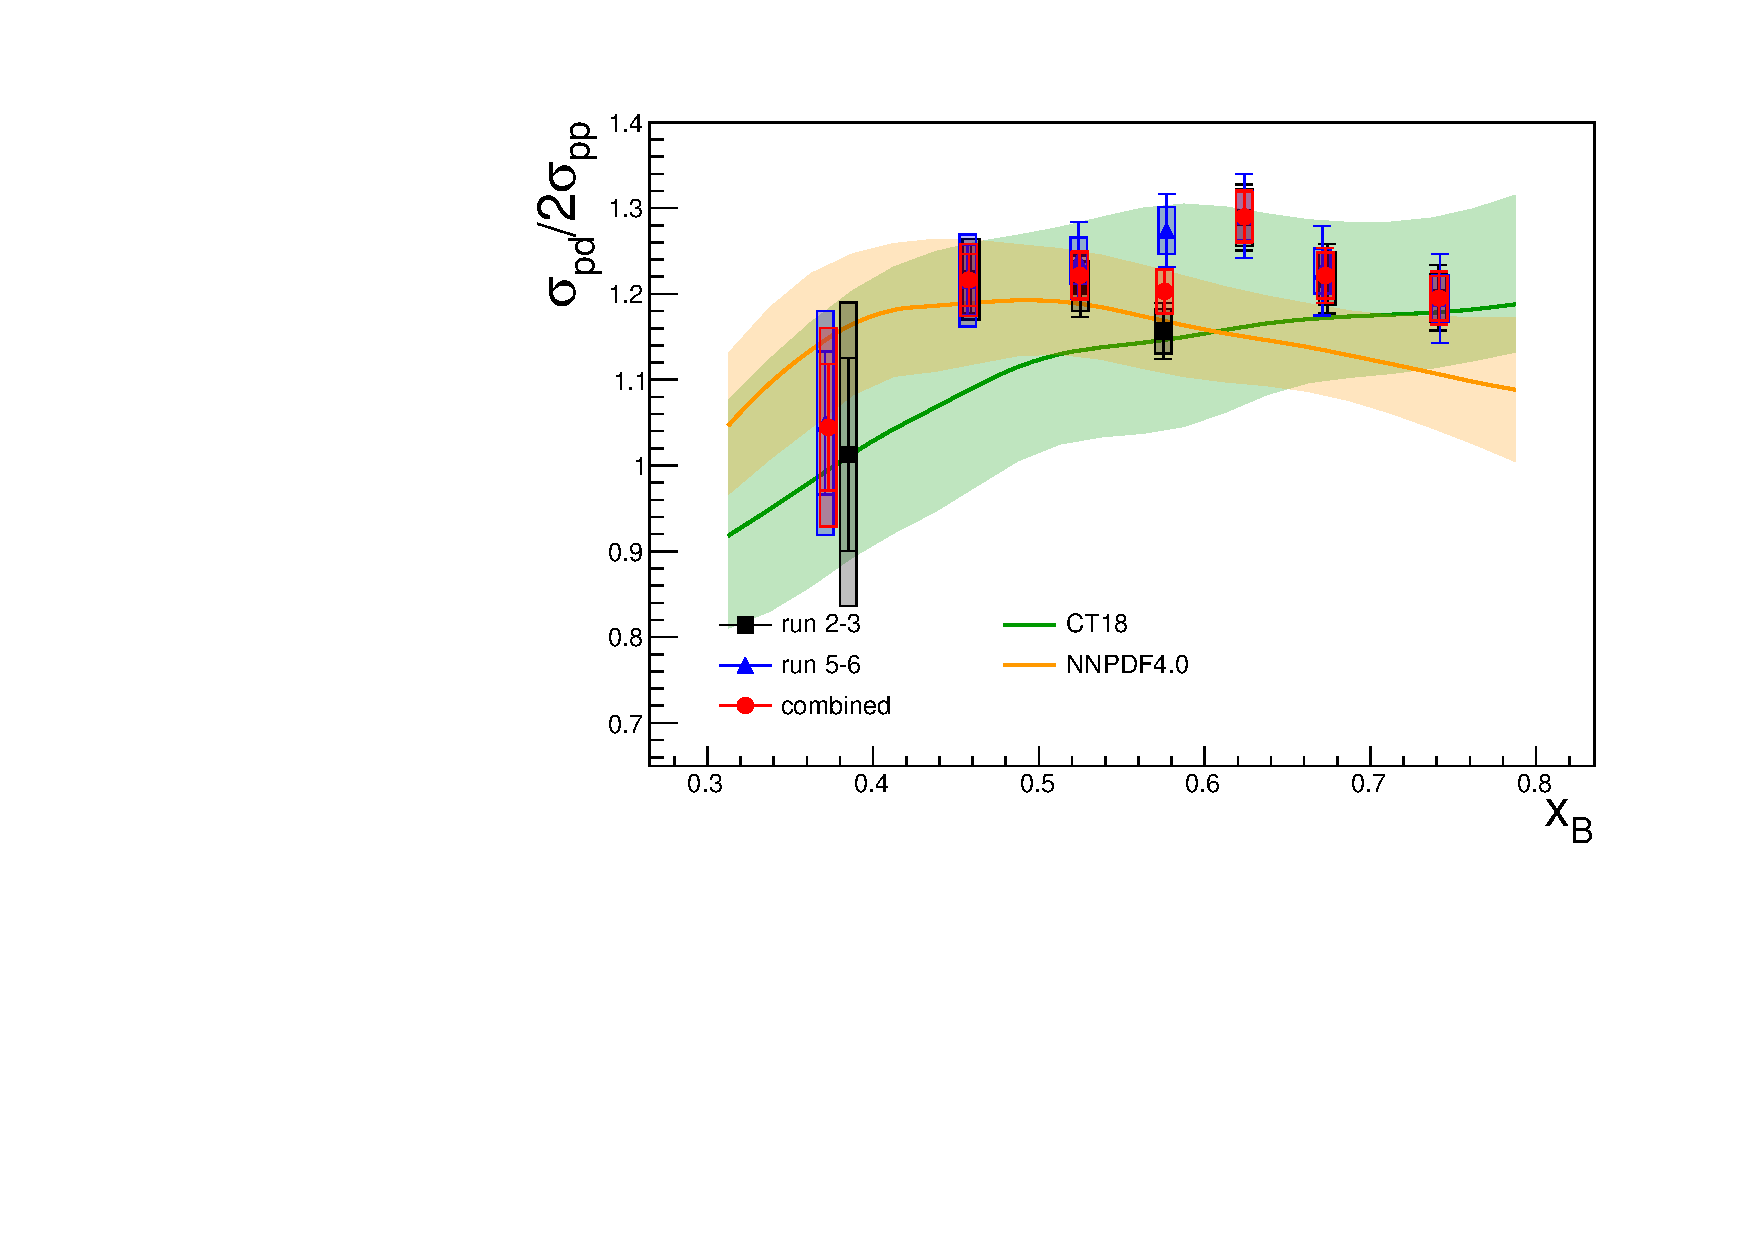
\includegraphics[width=0.7\linewidth]{DY-csr/MF_full_xB_syst.pdf}
	\caption{The extracted Drell-Yan cross section ratio as a function of $x_B$
		using the mass fit method from the two datasets and the combined analysis,
		and compared with calculations using CT18 and NNPDF4.0.}
	\label{fig:CSR_MF_xB}
\end{figure}
\begin{table}[htpb!]
	\centering
	\caption{The extracted Drell-Yan cross section ratio as a function of $x_B$ using the mass fit method.}
	\label{tab:DY-MF-x1}
	\begin{tabular}{c|ccc}
\hline
$x_B$ bin  & Run 2-3                 & Run 5-6                 & Combined                \\ \hline
$0.3-0.4$  & $1.013\pm0.112\pm0.177$ & $1.050\pm0.083\pm0.131$ & $1.045\pm0.074\pm0.116$ \\
$0.4-0.5$  & $1.217\pm0.040\pm0.047$ & $1.216\pm0.041\pm0.053$ & $1.216\pm0.030\pm0.042$ \\
$0.5-0.55$ & $1.209\pm0.036\pm0.029$ & $1.239\pm0.045\pm0.027$ & $1.222\pm0.028\pm0.026$ \\
$0.55-0.6$ & $1.157\pm0.033\pm0.026$ & $1.274\pm0.043\pm0.027$ & $1.203\pm0.026\pm0.025$ \\
$0.6-0.65$ & $1.289\pm0.038\pm0.033$ & $1.291\pm0.049\pm0.028$ & $1.290\pm0.030\pm0.029$ \\
$0.65-0.7$ & $1.218\pm0.040\pm0.030$ & $1.227\pm0.052\pm0.026$ & $1.221\pm0.032\pm0.027$ \\
$0.7-0.8$  & $1.195\pm0.038\pm0.028$ & $1.195\pm0.052\pm0.027$ & $1.195\pm0.031\pm0.026$ \\ \hline
\end{tabular}

\end{table}
\begin{figure}[htpb!]
	\centering
	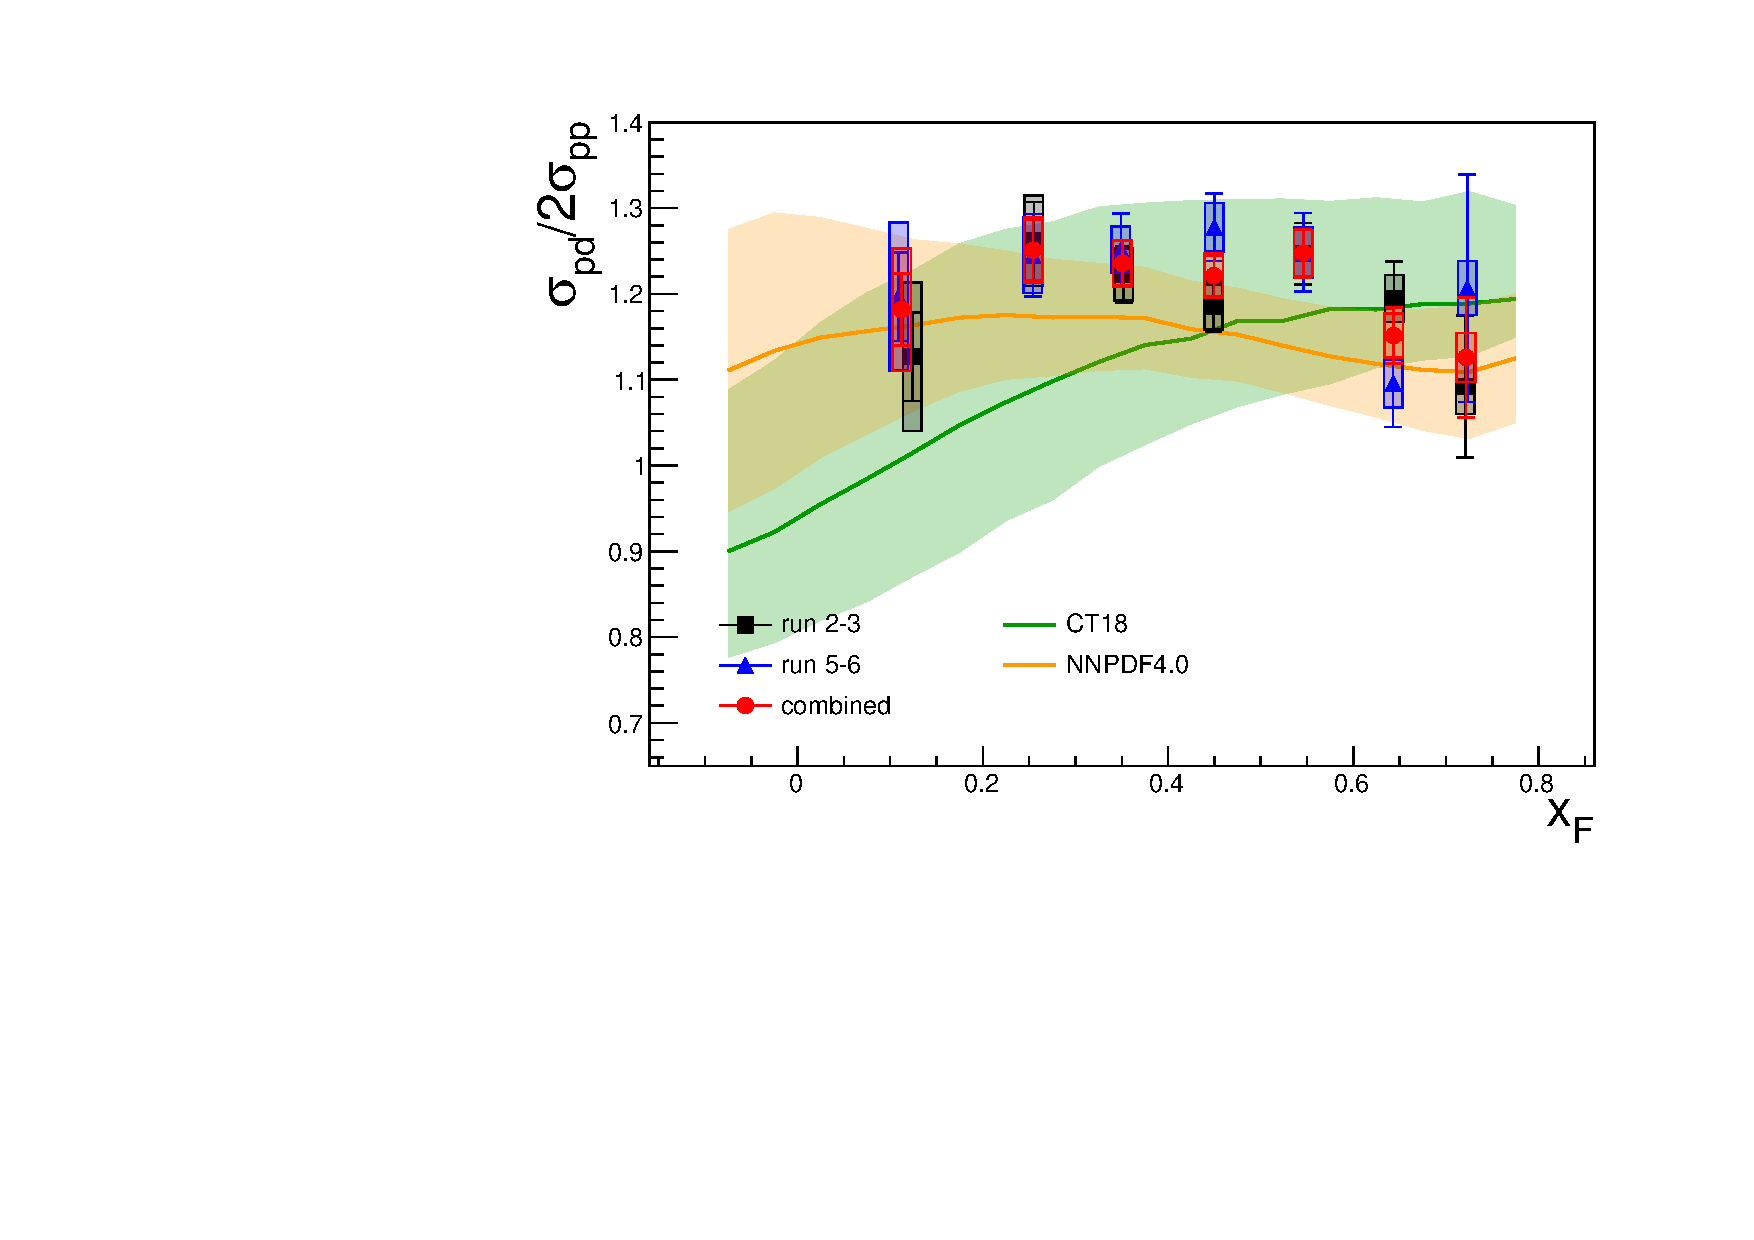
\includegraphics[width=0.7\linewidth]{DY-csr/MF_full_xF_syst.pdf}
	\caption{The extracted Drell-Yan cross section ratio as a function of $x_F$
		using the mass fit method from the two datasets and the combined analysis,
		and compared with calculations using CT18 and NNPDF4.0.}
	\label{fig:CSR_MF_xF}
\end{figure}
\begin{table}[htpb!]
	\centering
	\caption{The extracted Drell-Yan cross section ratio as a function of $x_F$ using the mass fit method.}
	\label{tab:DY-MF-xF}
	\begin{tabular}{c|ccc}
\hline
$x_F$ bin  & Run 2-3                 & Run 5-6                 & Combined                \\ \hline
$-0.1-0.2$ & $1.127\pm0.052\pm0.087$ & $1.197\pm0.052\pm0.086$ & $1.182\pm0.042\pm0.071$ \\
$0.2-0.3$  & $1.262\pm0.045\pm0.053$ & $1.245\pm0.048\pm0.044$ & $1.251\pm0.035\pm0.038$ \\
$0.3-0.4$  & $1.223\pm0.033\pm0.030$ & $1.252\pm0.042\pm0.027$ & $1.236\pm0.026\pm0.027$ \\
$0.4-0.5$  & $1.185\pm0.030\pm0.026$ & $1.278\pm0.039\pm0.028$ & $1.221\pm0.024\pm0.026$ \\
$0.5-0.6$  & $1.247\pm0.036\pm0.028$ & $1.248\pm0.046\pm0.029$ & $1.248\pm0.028\pm0.027$ \\
$0.6-0.7$  & $1.195\pm0.043\pm0.027$ & $1.096\pm0.051\pm0.028$ & $1.151\pm0.033\pm0.025$ \\
$0.7-0.8$  & $1.092\pm0.083\pm0.032$ & $1.207\pm0.133\pm0.031$ & $1.126\pm0.070\pm0.028$ \\ \hline
\end{tabular}

\end{table}
\FloatBarrier

\subsection{Comparison with global PDF analysis}
\Cref{fig:e866_e906} shows the comparison of the measured $\sigma_{pd}/2\sigma_{pp}$ from SeaQuest and NuSea~\cite{towell2001},
as well as calculations using CT18 PDFs. 
Part of the apparent difference between the measured $\sigma_{pd}/2\sigma_{pp}$ from the two experiment originates
from the different beam energies and therefore different $x_B$ coverage.
This effect is reflected in the calculated cross section ratios in \cref{fig:e866_e906}.
The measured ratios from SeaQuest are consistent with both NuSea results and calculations using CT18 PDFs
at low $x_T$. Since the high statistics data at low $x_T$ from NuSea were used to constrain
the CT18 PDFs, the good agreement reflects the consistency between NuSea and SeaQuest results
at the low $x_T$ region. 
In contrast, the SeaQuest results at higher $x_T$ are significantly larger than NuSea results and calculations using CT18 PDFs.
The CT18 PDFs, based on fits that include the NuSea data, show a drop of the cross section
at large $x_T$. No such drop is observed in the SeaQuest results.
\begin{figure}[htpb!]
	\centering
	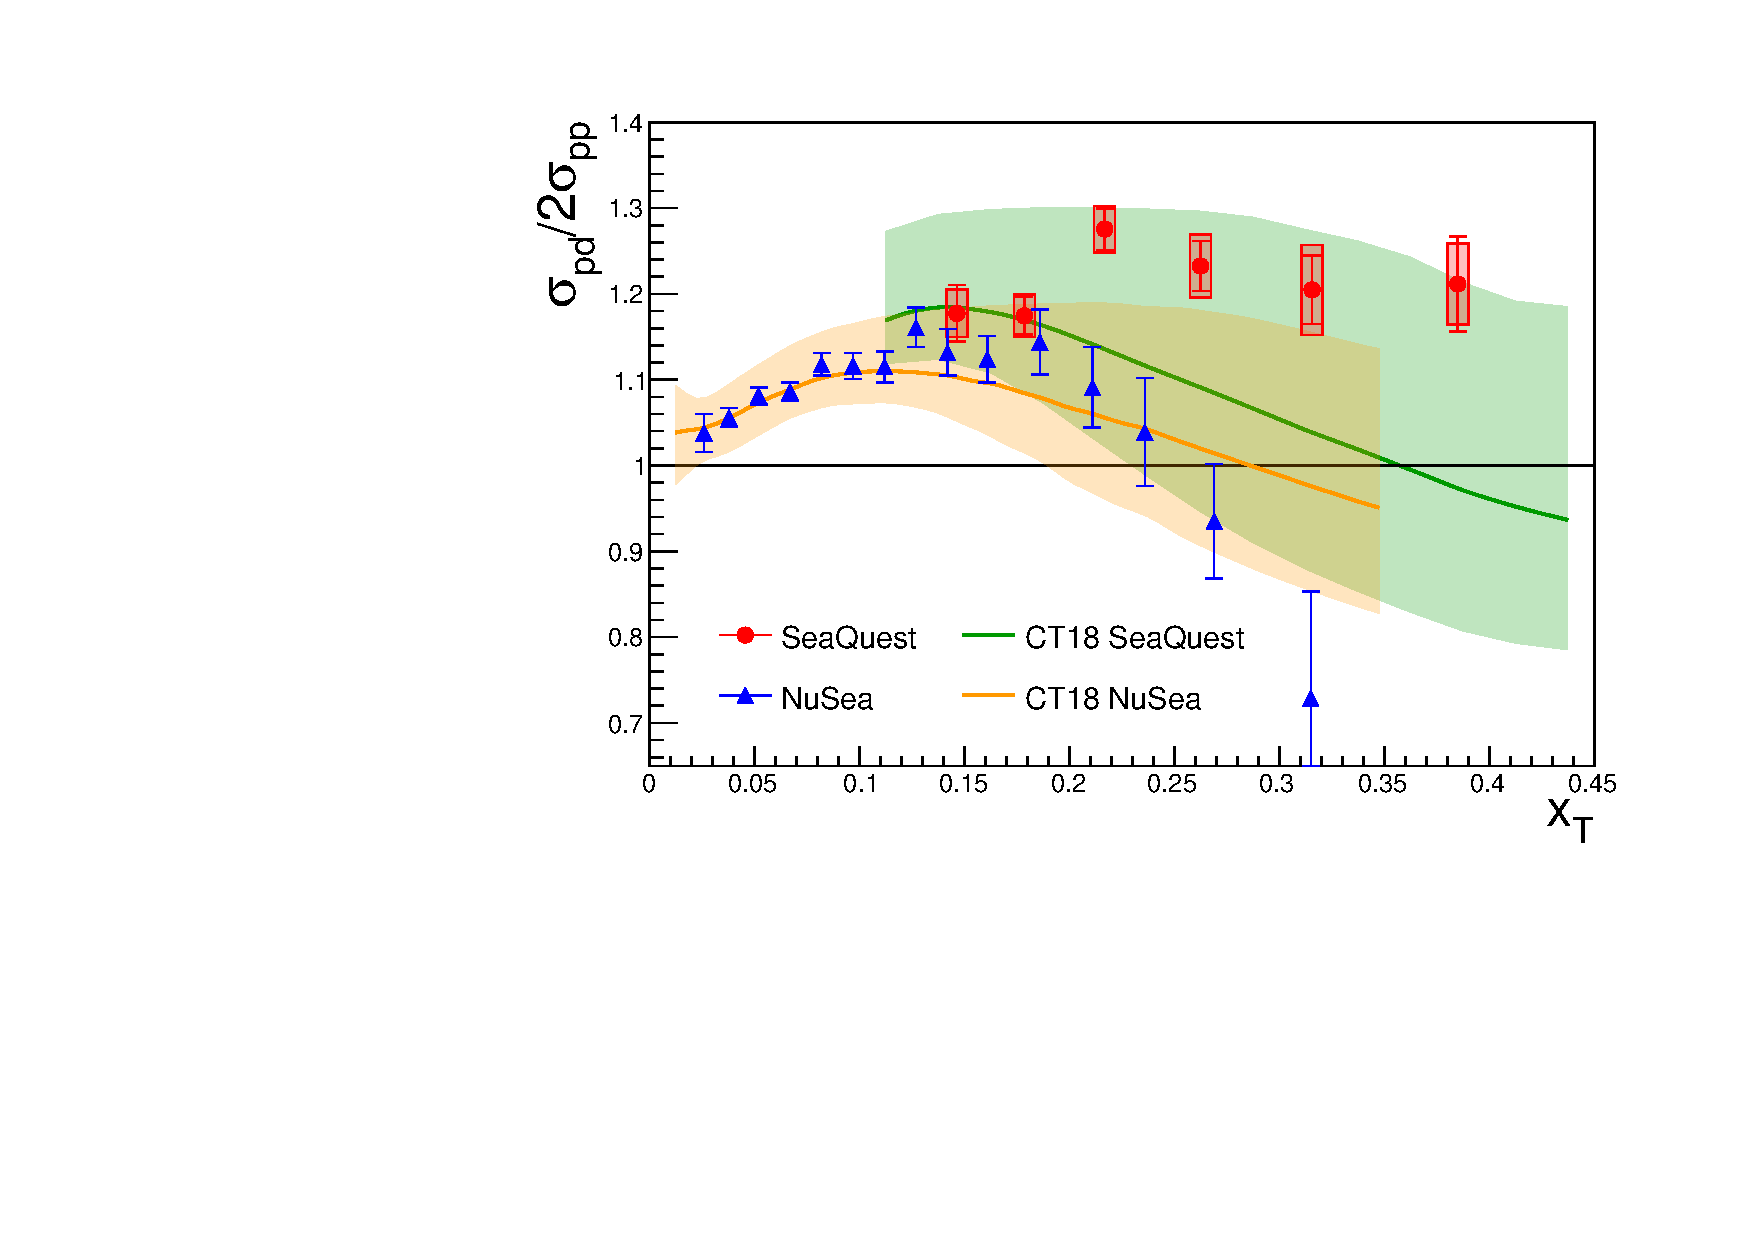
\includegraphics[width=0.8\linewidth]{DY-csr/E906_E866_xT_CT18only.pdf}
	\caption{The comparison of the measured $\sigma_{pd}/2\sigma_{pp}$ cross section ratios as function of $x_T$
		between SeaQuest (red circles) and NuSea~\cite{towell2001} (blue triangles).
		The curves represent calculations using CT18NLO~\cite{hou2021} at SeaQuest kinematics (green) and NuSea kinematics (orange).}
	\label{fig:e866_e906}
\end{figure} 

The published $\sigma_{pd}/2\sigma_{pp}$ ratio result using Run 2-3 data~\cite{dove2021,dove2023}
has been included in various recent global PDF analysis~\cite{cocuzza2021,guzzi2022,accardi2023,alekhin2023}.
In particular, \cref{fig:CSR_MF_xT} shows the calculation using CT18 (obtained without the SeaQuest data)
and NNPDF~4.0 (obtained with the SeaQuest data). The shift in the calculated cross section ratio is primarily
coming from the inclusion of the SeaQuest data.
As the NNPDF4.0 analysis were performed with the SeaQuest results in their global analysis,
calculations with NNPDF4.0 PDFs are naturally in better agreement with the SeaQuest results.

The importance of the SeaQuest data can be seen in the NNPDF4.0, where at large $x_T$, the
uncertainty band is consistent with the uncertainties of our measurements, as the SeaQuest
results is the only available data sensitive to the light sea-quark asymmetry at large $x$.
The updated $\sigma_{pd}/2\sigma_{pp}$ ratio from the combined analysis is slightly larger than the NNPDF4.0
calculation, this is partly due to the updated contamination correction, and partly due to the new data.
\begin{figure}[htpb!]
	\centering
	\begin{subfigure}{0.55\linewidth}
		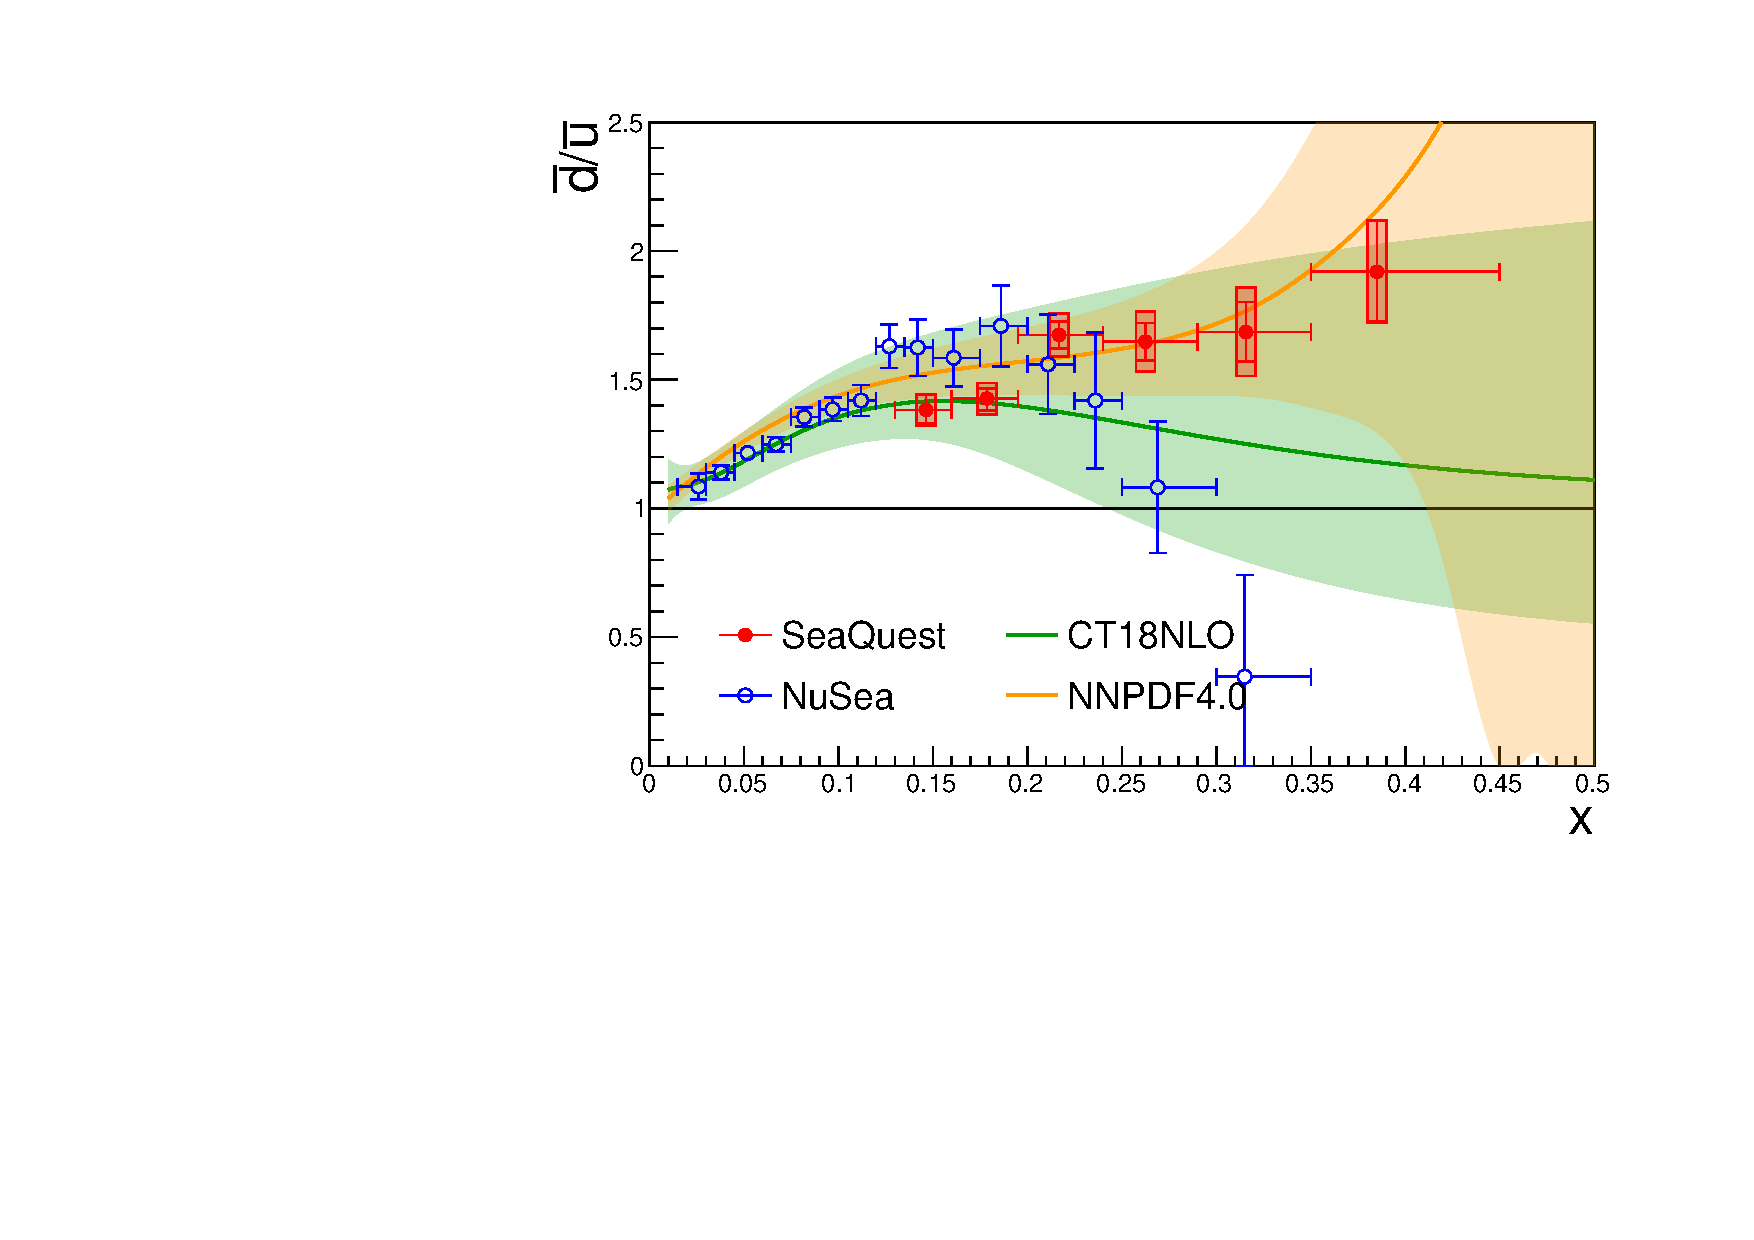
\includegraphics[width=\linewidth]{dbarUbar/E906_E866_dbarubar_PDF.pdf}
	\end{subfigure}
	\begin{subfigure}{0.55\linewidth}
		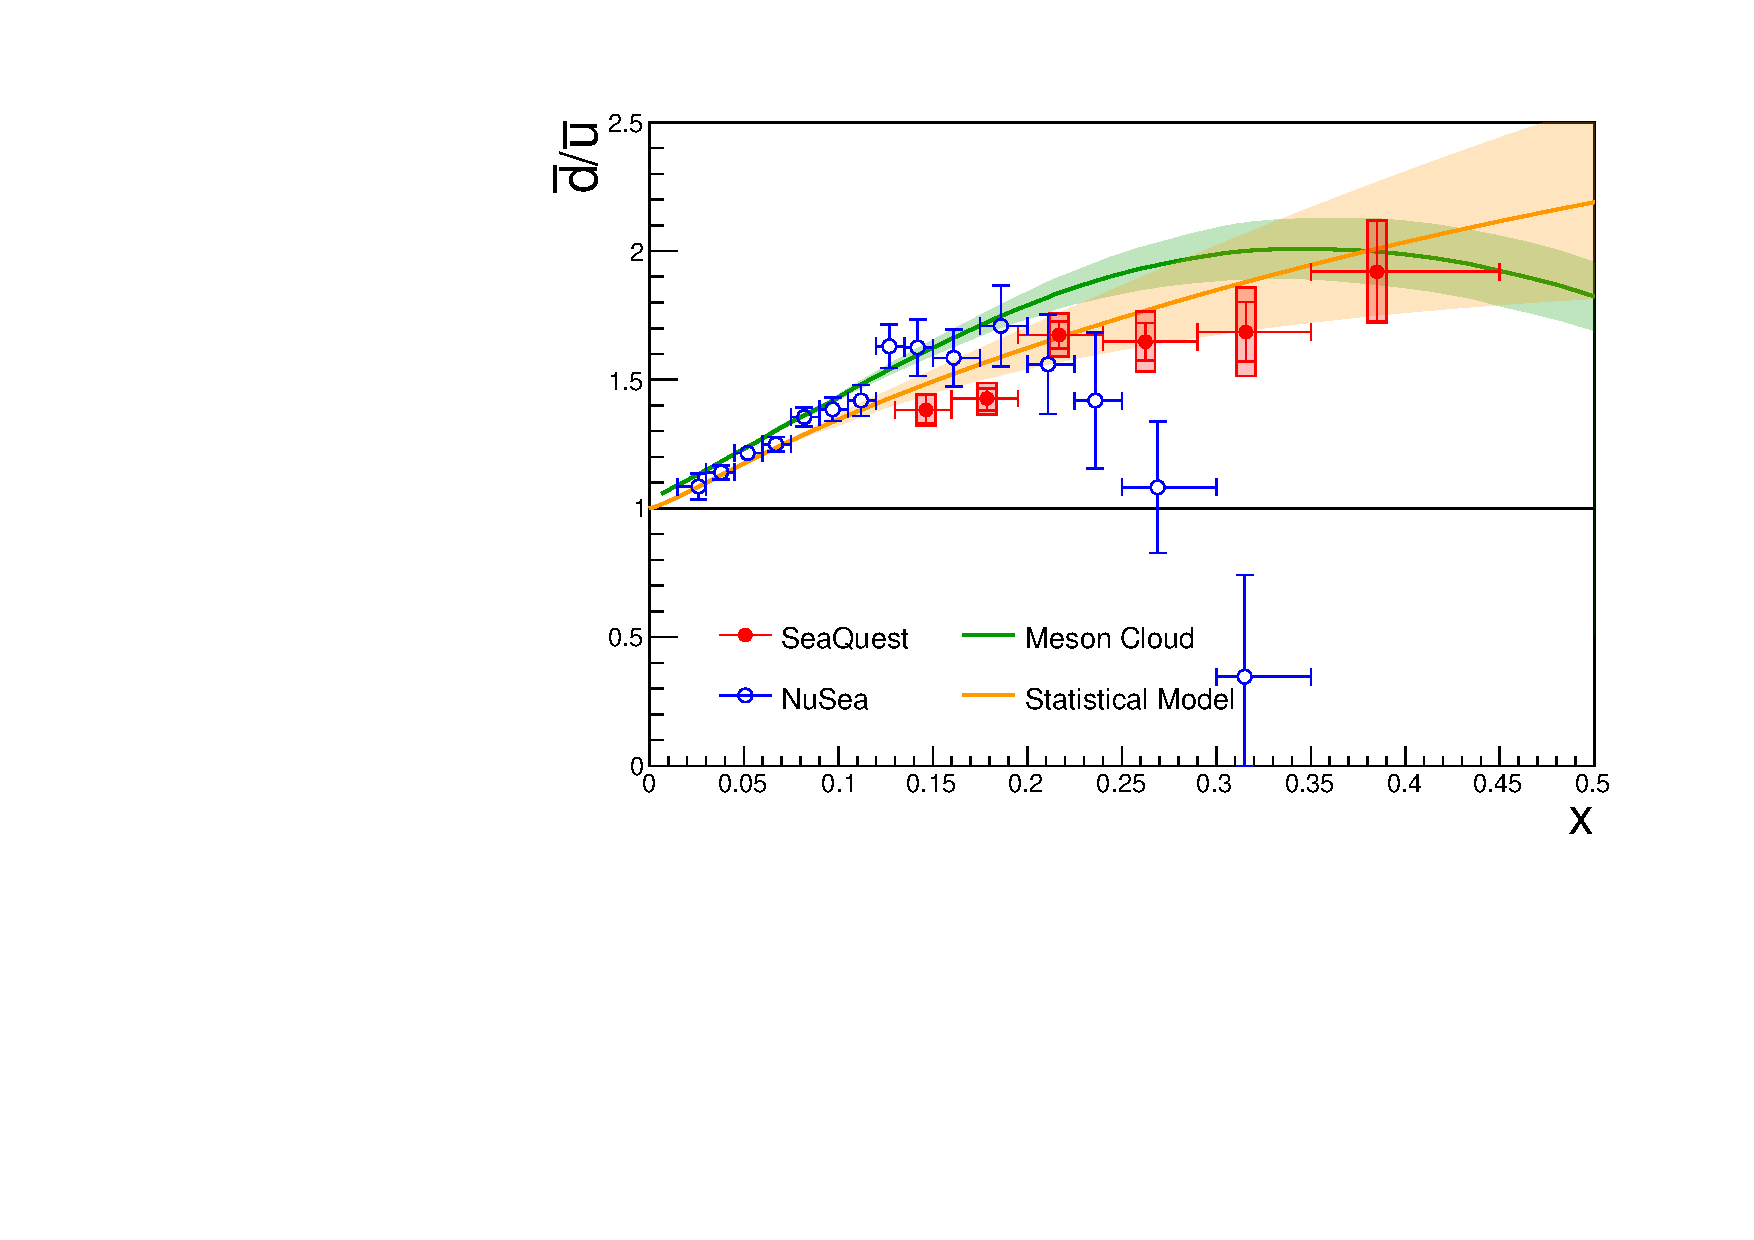
\includegraphics[width=\linewidth]{dbarUbar/E906_E866_dbarubar.pdf}
	\end{subfigure}
	\caption{The extracted $\bar{d}/\bar{u}$ from the measured $\sigma_{pd}/2\sigma_{pp}$ Drell-Yan cross section ratio
		from SeaQuest (red solid circles) and E866~\cite{towell2001} (open blue circles).
		The extracted ratios are compared with CT18~\cite{hou2021} and NNPDF4.0~\cite{ball2022a} global PDF analyses (top)
		and with predictions from meson cloud model~\cite{alberg2022} and statistical model~\cite{soffer2019} (bottom).}
	\label{fig:e906_e866_dbarubar}
\end{figure}
\begin{table}[htpb!]
	\centering
	\caption{The extracted $\bar{d}/\bar{u}$ for each $x$ bin. The first uncertainty is statistical the second systematic.}
	\label{tab:dbarubar_e906}
	\begin{tabular}{ccc}
\hline
$x$ range     & $\expval{x}$ & $\bar{d}/\bar{u}$                     \\ \hline
$0.130-0.160$ & $0.146$      & $1.383^{+0.058+0.060}_{-0.053-0.060}$ \\
$0.161-0.201$ & $0.181$      & $1.431^{+0.041+0.061}_{-0.051-0.061}$ \\
$0.202-0.242$ & $0.222$      & $1.672^{+0.052+0.082}_{-0.052-0.082}$ \\
$0.243-0.293$ & $0.263$      & $1.653^{+0.073+0.123}_{-0.073-0.113}$ \\
$0.294-0.354$ & $0.324$      & $1.694^{+0.124+0.174}_{-0.114-0.174}$ \\
$0.355-0.455$ & $0.395$      & $1.925^{+0.205+0.205}_{-0.195-0.205}$ \\ \hline
\end{tabular}

\end{table}

In order to compared the results from SeaQuest with predictions from various models,
an estimate for the $\bar{d}/\bar{u}$ ratio is extracted from the cross section ratio by
an iterative method, as described in Ref.~\cite{dove2021}. 
We first make an estimate for the $\bar{d}/\bar{u}$ ratio over the measured $x_T$
and calculate the cross section ratio $R$ using a chosen PDF set. 
This PDF set provides all other parton distributions except for the $\bar{d}/\bar{u}$ ratio,
which is allowed to vary. The $\bar{d}/\bar{u}$ ratio is initialized as 
\begin{equation}
	\left[\frac{\bar{d}}{\bar{u}}\right]\left(x_T\right) = 2R\left(x_T\right)-1.
\end{equation}
The $\bar{d}/\bar{u}$ ratio outside the measured $x_T$ range was assumed to be $1.0$,
and change to $0.5$ and $2.0$ to estimate the systematic uncertainty arises from this assumption.
The cross section ratio $R$ is then calculated up to next-to-leading order, as 
\begin{equation}
	R_{\mathrm{pred}}\left(x_T\right)  = \frac{\sum_{x_B} A\left(x_B, x_T\right)\sigma^{pd}_{NLO}\left(x_B, x_T\right)}{2\sum_{x_B} A\left(x_B, x_T\right)\sigma^{pp}_{NLO}\left(x_B, x_T\right)},
\end{equation}
where $A\left(x_B,x_T\right)$ is the acceptance for a $\left(x_B, x_T\right)$ bin. 
The $\bar{d}/\bar{u}$ ratio is then adjusted according the to the difference between
the measured and predicted ratios, until the difference is less then $10^{-3}$.

The extracted $\bar{d}/\bar{u}$ from the measured SeaQuest cross section ratio,
using the CT18 PDFs as the basis, are shown in \cref{fig:e906_e866_dbarubar} 
and tabulated in \cref{tab:dbarubar_e906}. 
While the SeaQuest results are consistent with previous E866 results~\cite{towell2001} at low $x$,
the extracted $\bar{d}/\bar{u}$ ratios from the SeaQuest measurements continue to rise as $x$ increases,
and is in tension with the E866 result.
The SeaQuest results are also in much better agreement with predictions from meson cloud model~\cite{alberg2022}
and statistical model~\cite{soffer2019}.
The extracted $\bar{d}/\bar{u}$ ratios are also compared with results from CT18~\cite{hou2021} and NNPDF4.0~\cite{ball2022a}
global analyses in \cref{fig:e906_e866_dbarubar}. 
The inclusion of the SeaQuest result from Run 2-3 in the NNPDF4.0 analysis strongly constrains the $\bar{d}/\bar{u}$ ratios
to remain above unity at large $x$.
With the reduced statistical uncertainties from the combined analysis,
the uncertainty on the $\bar{d}/\bar{u}$ in these global analyses can be further reduced.
\begin{comment}
The impact of the SeaQuest measurement is further illustrated in \cref{fig:JAM_impact}. 
The JAM analysis~\cite{cocuzza2021} found that the SeaQuest measurement greatly reduces the 
uncertainties on the $\bar{d}/\bar{u}$ ratio, by up to $\approx 50\%$ at $x>0.3$. 
The addition of the SeaQuest data also constrain the ratio to remain above unity up to values of $x\approx0.4$,
which is also in better agreement with prediction from various models, including meson-cloud and statistical model.
\begin{figure}[h!]
	\centering
	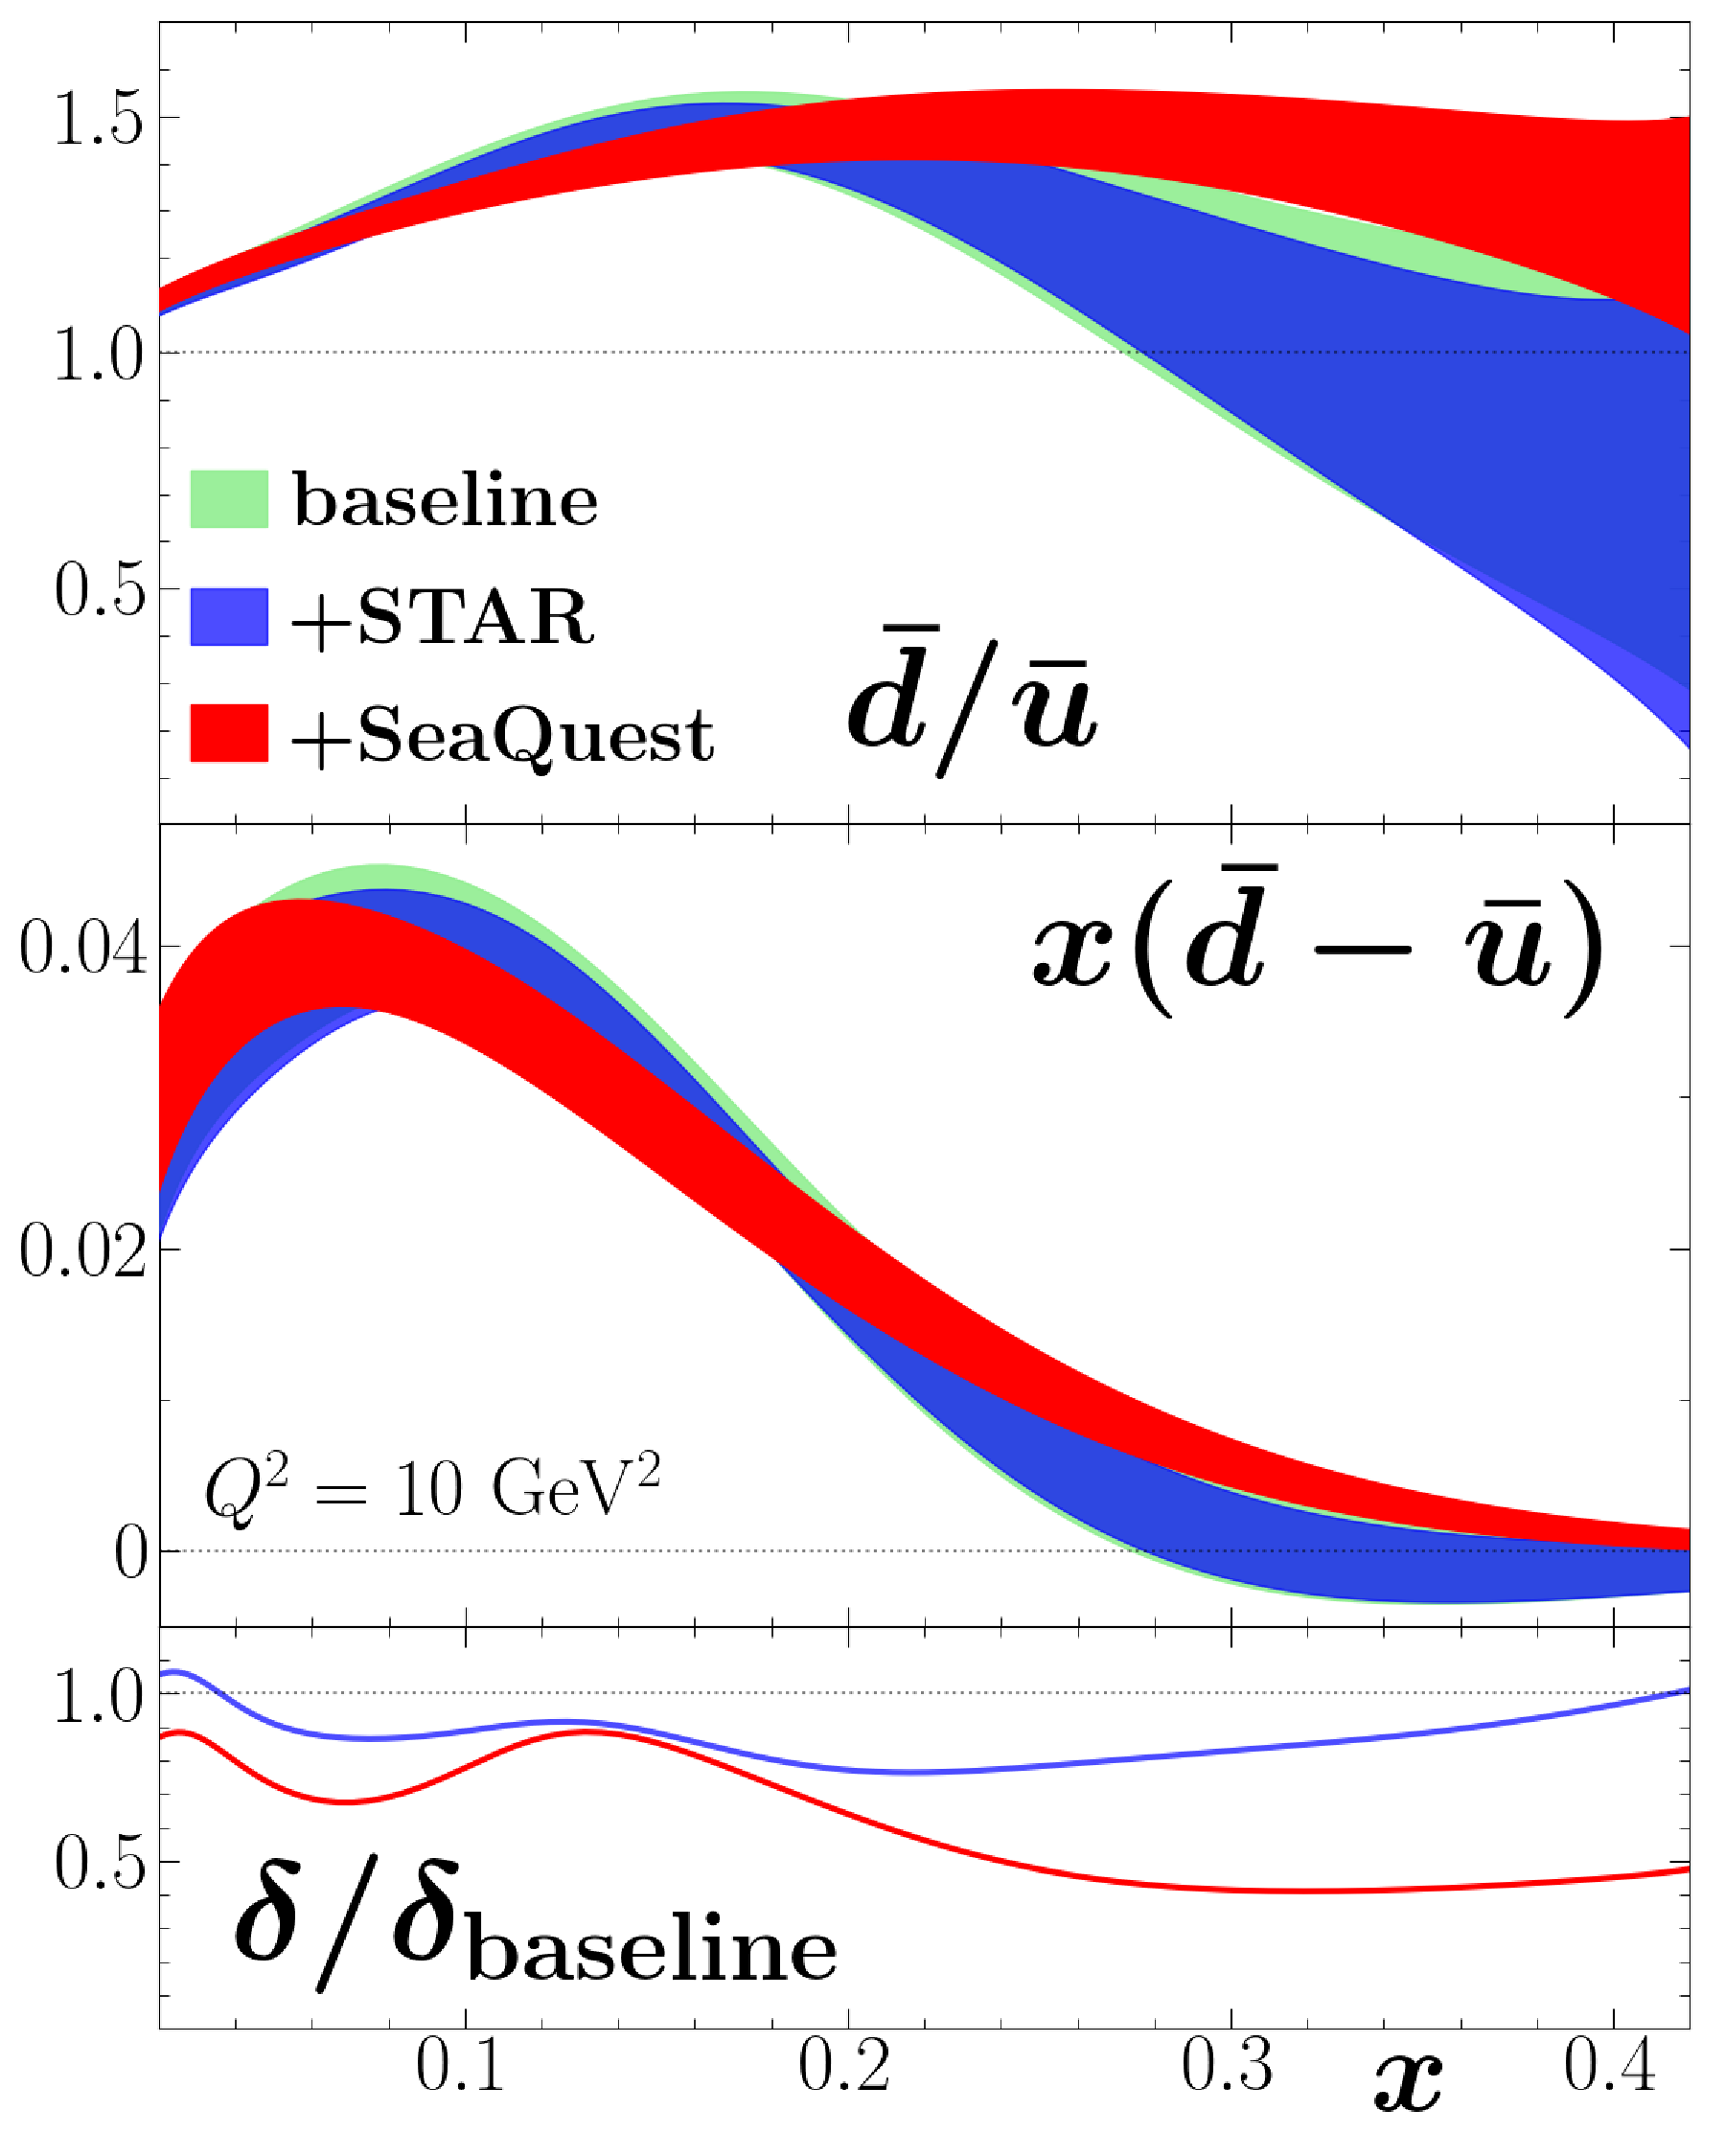
\includegraphics[width=0.5\linewidth]{JAM_impact}
	\caption{impact on the $\bar{d}/\bar{u}$ ratio (top) and the asymmetry $x\left(\bar{d}-\bar{u}\right)$ (middle)
		of the SeaQuest measurement (red band) and STAR $W$ data \cite{adam2021} (blue band) relative to the baseline (green band) 
		where the SeaQuest and STAR measurements are excluded in the JAM analysis~\cite{cocuzza2021}.
		The uncertainty on $\bar{d}/\bar{u}$ for these two scenarios normalized to that of the baseline
		are shown in the bottom panel. Taken from Ref.~\cite{cocuzza2021}.}
	\label{fig:JAM_impact}
\end{figure}
\end{comment}

\subsection{Comparison between Massfit and Intensity Extrapolation Method}
As described in \cref{M-sec:extrapolation}, an independent method for extracting the Drell-Yan cross section
ratio is developed by utilizing its rate dependence. 

\subsubsection{Systematic uncertainties due to choice of fit function}
To understand the systematic uncertainties in the intensity extrapolation method due to the
choice of fit function, the following two fit functions are used.
\begin{align}
	R_i\left(I\right) & = p_{0i} + p_{1} I + p_{2} I^2 \quad\text{(FIT 1)}                                                     \\
	R_i\left(I\right) & = p_{0i} + \left[p_{10} + p_{11}x_i\right] I + \left[p_{20} + p_{21}x_i\right]I^2 \quad \text{(FIT 2)}
	\label{eq:fit_functions}
\end{align}
The fit to data using the two fits for selected $x_T$ bins are shown in \cref{fig:FIT1_selected,fig:FIT2_selected},
and $\chi^2$ for the fits are tabulated in \cref{tab:chi_IE}.
The fit in other $x_T$ bins and for other variables are shown in \cref{M-a_ch:extrapolation}.
%\begin{figure}
	\centering
	\caption{Fit to the flask subtracted yield ratio with FIT1 for $x_T$ for run 2-3.}
	\label{fig:run2-3_FIT1_xT}
	\begin{subfigure}{0.45\linewidth}
		\includegraphics[width=\linewidth]{extrapolation/run2-3/xT/FIT1/hist_fitted_xT_tInt_0}
	\end{subfigure}
	\begin{subfigure}{0.45\linewidth}
		\includegraphics[width=\linewidth]{extrapolation/run2-3/xT/FIT1/hist_fitted_xT_tInt_1}
	\end{subfigure}
	\begin{subfigure}{0.45\linewidth}
		\includegraphics[width=\linewidth]{extrapolation/run2-3/xT/FIT1/hist_fitted_xT_tInt_2}
	\end{subfigure}
	\begin{subfigure}{0.45\linewidth}
		\includegraphics[width=\linewidth]{extrapolation/run2-3/xT/FIT1/hist_fitted_xT_tInt_3}
	\end{subfigure}
	\begin{subfigure}{0.45\linewidth}
		\includegraphics[width=\linewidth]{extrapolation/run2-3/xT/FIT1/hist_fitted_xT_tInt_4}
	\end{subfigure}
	\begin{subfigure}{0.45\linewidth}
		\includegraphics[width=\linewidth]{extrapolation/run2-3/xT/FIT1/hist_fitted_xT_tInt_5}
	\end{subfigure}
\end{figure}

%\begin{figure}
	\centering
	\caption{Fit to the flask subtracted yield ratio with FIT2 for $x_T$ for run 2-3.}
	\label{fig:run2-3_FIT2_xT}
	\begin{subfigure}{0.45\linewidth}
		\includegraphics[width=\linewidth]{extrapolation/run2-3/xT/FIT2/hist_fitted_xT_tInt_0}
	\end{subfigure}
	\begin{subfigure}{0.45\linewidth}
		\includegraphics[width=\linewidth]{extrapolation/run2-3/xT/FIT2/hist_fitted_xT_tInt_1}
	\end{subfigure}
	\begin{subfigure}{0.45\linewidth}
		\includegraphics[width=\linewidth]{extrapolation/run2-3/xT/FIT2/hist_fitted_xT_tInt_2}
	\end{subfigure}
	\begin{subfigure}{0.45\linewidth}
		\includegraphics[width=\linewidth]{extrapolation/run2-3/xT/FIT2/hist_fitted_xT_tInt_3}
	\end{subfigure}
	\begin{subfigure}{0.45\linewidth}
		\includegraphics[width=\linewidth]{extrapolation/run2-3/xT/FIT2/hist_fitted_xT_tInt_4}
	\end{subfigure}
	\begin{subfigure}{0.45\linewidth}
		\includegraphics[width=\linewidth]{extrapolation/run2-3/xT/FIT2/hist_fitted_xT_tInt_5}
	\end{subfigure}
\end{figure}

\begin{figure}[h!]
	\centering
	\begin{subfigure}{0.45\linewidth}
		\includegraphics[width=\linewidth]{extrapolation/run2-3/xT/FIT1/hist_fitted_xT_tInt_0}
	\end{subfigure}
	\begin{subfigure}{0.45\linewidth}
		\includegraphics[width=\linewidth]{extrapolation/run5-6/xT/FIT1/hist_fitted_xT_tInt_0}
	\end{subfigure}
	\begin{subfigure}{0.45\linewidth}
		\includegraphics[width=\linewidth]{extrapolation/run2-3/xT/FIT1/hist_fitted_xT_tInt_2}
	\end{subfigure}
	\begin{subfigure}{0.45\linewidth}
		\includegraphics[width=\linewidth]{extrapolation/run5-6/xT/FIT1/hist_fitted_xT_tInt_2}
	\end{subfigure}
	\begin{subfigure}{0.45\linewidth}
		\includegraphics[width=\linewidth]{extrapolation/run2-3/xT/FIT1/hist_fitted_xT_tInt_3}
	\end{subfigure}
	\begin{subfigure}{0.45\linewidth}
		\includegraphics[width=\linewidth]{extrapolation/run5-6/xT/FIT1/hist_fitted_xT_tInt_3}
	\end{subfigure}
	\caption{Fit to the flask subtracted yield ratio with FIT1 for $x_T$ for run 2-3 (left) and run 5-6 (right)in odd numbered $x_T$ bins.}
	\label{fig:FIT1_selected}
\end{figure}
\begin{figure}[h!]
	\centering
	\begin{subfigure}{0.45\linewidth}
		\includegraphics[width=\linewidth]{extrapolation/run2-3/xT/FIT2/hist_fitted_xT_tInt_0}
	\end{subfigure}
	\begin{subfigure}{0.45\linewidth}
		\includegraphics[width=\linewidth]{extrapolation/run5-6/xT/FIT2/hist_fitted_xT_tInt_0}
	\end{subfigure}
	\begin{subfigure}{0.45\linewidth}
		\includegraphics[width=\linewidth]{extrapolation/run2-3/xT/FIT2/hist_fitted_xT_tInt_2}
	\end{subfigure}
	\begin{subfigure}{0.45\linewidth}
		\includegraphics[width=\linewidth]{extrapolation/run5-6/xT/FIT2/hist_fitted_xT_tInt_2}
	\end{subfigure}
	\begin{subfigure}{0.45\linewidth}
		\includegraphics[width=\linewidth]{extrapolation/run2-3/xT/FIT2/hist_fitted_xT_tInt_3}
	\end{subfigure}
	\begin{subfigure}{0.45\linewidth}
		\includegraphics[width=\linewidth]{extrapolation/run5-6/xT/FIT2/hist_fitted_xT_tInt_3}
	\end{subfigure}
	\caption{Fit to the flask subtracted yield ratio with FIT2 for $x_T$ for run 2-3 (left) and run 5-6 (right)in odd numbered $x_T$ bins.}
	\label{fig:FIT2_selected}
\end{figure}

\begin{figure}[h!]
	\centering
	\begin{subfigure}{0.6\linewidth}
		\includegraphics*[width=\linewidth]{DY-csr/run23_xT_IE}
	\end{subfigure}\\
	\begin{subfigure}{0.45\linewidth}
		\includegraphics*[width=\linewidth]{DY-csr/run23_xB_IE}
	\end{subfigure}
	\begin{subfigure}{0.45\linewidth}
		\includegraphics*[width=\linewidth]{DY-csr/run23_xF_IE}
	\end{subfigure}
	\caption{Comparison of the extracted Drell-Yan cross section ratio as a function of $x_T$(top),
		$x_B$(left) and $x_F$(right) using the intensity extrapolation method with the two fit functions in \cref{eq:fit_functions}
		using Run 2-3 data.}
	\label{fig:CSR_IE_run23}
\end{figure}

\begin{figure}[h!]
	\centering
	\begin{subfigure}{0.6\linewidth}
		\includegraphics*[width=\linewidth]{DY-csr/run56_xT_IE}
	\end{subfigure}\\
	\begin{subfigure}{0.45\linewidth}
		\includegraphics*[width=\linewidth]{DY-csr/run56_xB_IE}
	\end{subfigure}
	\begin{subfigure}{0.45\linewidth}
		\includegraphics*[width=\linewidth]{DY-csr/run56_xF_IE}
	\end{subfigure}
	\caption{Comparison of the extracted Drell-Yan cross section ratio as a function of $x_T$(top),
		$x_B$(left) and $x_F$(right) using the intensity extrapolation method with the two fit functions in \cref{eq:fit_functions}
		using Run 5-6 data.}
	\label{fig:CSR_IE_run56}
\end{figure}

While the difference caused by the fit functions are small for $x_T$ in Run 2-3,
as shown in \cref{fig:CSR_IE_run23} and reported in Ref.~\cite{dove2021},
the difference is significantly larger in the other variables and in Run 5-6, as shown in \cref{fig:CSR_IE_run56}.
This is a major systematic uncertainty in this method. 
In Ref.~\cite{dove2021}, Fit-1 was chosen as the central value, but the reduced $\chi^2$ are very similar between the two fits,
as tabulated in \cref{tab:chi_IE}. 
It should also be noted that during the Run 5-6 data taking, the variation in the instantaneous beam
intensity was reduced as compared to Run 2-3.
This is partly due to the improvement in beam quality and partly due to the tightening of the beam inhibit thresholds.
Therefore, the range of trigger intensity that can be used for the intensity extrapolation is smaller in Run 5-6. 
The smaller range might be partly responsible for the larger systematic uncertainty in the intensity extrapolation method
in Run 5-6.
\begin{table}[h!]
	\centering
	\caption{The reduced $\chi^2$ for the different fits used in the intensity extrapolation method for Run 2-3 and Run 5-6. }
	\label{tab:chi_IE}
	\begin{tabular}{c|ccc|ccc}
\hline
      & \multicolumn{3}{c|}{Run 2-3}                     & \multicolumn{3}{c}{Run 5-6}                      \\ \cline{2-7} 
      & $x_T$          & $x_B$          & $x_F$          & $x_T$          & $x_B$          & $x_F$          \\ \hline
FIT 1 & $40.1167 / 40$ & $71.3796 / 47$ & $68.0593 / 47$ & $18.7745 / 28$ & $42.0641 / 33$ & $29.6759 / 33$ \\ \hline
FIT 2 & $40.008 / 38$  & $61.8549 / 45$ & $64.1524 / 45$ & $16.9269 / 26$ & $40.4342 / 31$ & $27.3795 / 31$ \\ \hline
\end{tabular}
\end{table}

\subsubsection{Results from Intensity Extrapolation method.}
The extracted ratios using this method are shown in \cref{fig:CSR_IE},
and are tabulated in \cref{tab:DY-IE-x2,tab:DY-IE-x1,tab:DY-IE-xF}.
\begin{figure}[h!]
	\centering
	\begin{subfigure}{0.6\linewidth}
		\includegraphics*[width=\linewidth]{DY-csr/IE_full_xT_syst}
	\end{subfigure}\\
	\begin{subfigure}{0.45\linewidth}
		\includegraphics*[width=\linewidth]{DY-csr/IE_full_xB_syst}
	\end{subfigure}
	\begin{subfigure}{0.45\linewidth}
		\includegraphics*[width=\linewidth]{DY-csr/IE_full_xF_syst}
	\end{subfigure}
	\caption{Comparison of the extracted Drell-Yan cross section ratio as a function of $x_T$(top),
		$x_B$(left) and $x_F$(right) using the intensity extrapolation method from the two datasets.}
	\label{fig:CSR_IE}
\end{figure}

\begin{table}[h!]
	\centering
	\caption{The extracted Drell-Yan cross section ratio as a function of $x_T$ using the intensity extrapolation method.}
	\label{tab:DY-IE-x2}
	\begin{tabular}{c|ccc}
\hline
$x_T$ bin    & Run 2-3                 & Run 5-6                 & Combined                \\ \hline
$0.13-0.16$  & $1.227\pm0.051\pm0.047$ & $0.995\pm0.066\pm0.109$ & $1.113\pm0.042\pm0.061$ \\
$0.16-0.195$ & $1.157\pm0.043\pm0.025$ & $1.076\pm0.057\pm0.040$ & $1.127\pm0.034\pm0.027$ \\
$0.195-0.24$ & $1.212\pm0.042\pm0.046$ & $1.195\pm0.059\pm0.042$ & $1.204\pm0.036\pm0.036$ \\
$0.24-0.29$  & $1.181\pm0.046\pm0.034$ & $1.144\pm0.060\pm0.033$ & $1.165\pm0.037\pm0.029$ \\
$0.29-0.35$  & $1.209\pm0.049\pm0.035$ & $1.097\pm0.067\pm0.052$ & $1.163\pm0.040\pm0.034$ \\
$0.35-0.45$  & $1.129\pm0.063\pm0.038$ & $1.118\pm0.079\pm0.097$ & $1.124\pm0.049\pm0.050$ \\ \hline
\end{tabular}


\end{table}
\begin{table}[h!]
	\centering
	\caption{The extracted Drell-Yan cross section ratio as a function of $x_B$ using the intensity extrapolation method.}
	\label{tab:DY-IE-x1}
	\begin{tabular}{c|ccc}
\hline
$x_B$ bin  & Run 2-3                 & Run 5-6                 & Combined                \\ \hline
$0.3-0.4$  & $1.044\pm0.062\pm0.180$ & $0.925\pm0.078\pm0.088$ & $0.942\pm0.067\pm0.081$ \\
$0.4-0.5$  & $1.214\pm0.044\pm0.110$ & $1.086\pm0.055\pm0.058$ & $1.110\pm0.046\pm0.053$ \\
$0.5-0.55$ & $1.178\pm0.045\pm0.054$ & $1.098\pm0.063\pm0.032$ & $1.136\pm0.039\pm0.035$ \\
$0.55-0.6$ & $1.147\pm0.043\pm0.023$ & $1.145\pm0.060\pm0.045$ & $1.146\pm0.035\pm0.027$ \\
$0.6-0.65$ & $1.241\pm0.047\pm0.065$ & $1.185\pm0.065\pm0.045$ & $1.209\pm0.043\pm0.041$ \\
$0.65-0.7$ & $1.200\pm0.050\pm0.095$ & $1.091\pm0.066\pm0.066$ & $1.122\pm0.049\pm0.056$ \\
$0.7-0.8$  & $1.176\pm0.047\pm0.140$ & $1.016\pm0.068\pm0.106$ & $1.044\pm0.056\pm0.092$ \\ \hline
\end{tabular}

\end{table}
\begin{table}[h!]
	\centering
	\caption{The extracted Drell-Yan cross section ratio as a function of $x_F$ using the intensity extrapolation method.}
	\label{tab:DY-IE-xF}
	\begin{tabular}{c|ccc}
\hline
$x_F$ bin  & Run 2-3                 & Run 5-6                 & Combined                \\ \hline
$-0.1-0.2$ & $1.139\pm0.047\pm0.128$ & $1.094\pm0.062\pm0.105$ & $1.102\pm0.052\pm0.091$ \\
$0.2-0.3$  & $1.209\pm0.047\pm0.072$ & $1.078\pm0.060\pm0.062$ & $1.124\pm0.042\pm0.050$ \\
$0.3-0.4$  & $1.189\pm0.044\pm0.039$ & $1.124\pm0.062\pm0.032$ & $1.161\pm0.036\pm0.031$ \\
$0.4-0.5$  & $1.170\pm0.041\pm0.029$ & $1.155\pm0.060\pm0.038$ & $1.164\pm0.034\pm0.028$ \\
$0.5-0.6$  & $1.211\pm0.047\pm0.071$ & $1.093\pm0.062\pm0.071$ & $1.137\pm0.043\pm0.054$ \\
$0.6-0.7$  & $1.189\pm0.051\pm0.094$ & $0.962\pm0.068\pm0.138$ & $1.030\pm0.050\pm0.102$ \\
$0.7-0.8$  & $0.912\pm0.074\pm0.134$ & $0.951\pm0.118\pm0.159$ & $0.936\pm0.078\pm0.112$ \\ \hline
\end{tabular}

\end{table}
\FloatBarrier

\begin{figure}[h!]
	\centering
	\begin{subfigure}{0.6\linewidth}
		\includegraphics*[width=\linewidth]{DY-csr/method_full_xT_syst}
	\end{subfigure}\\
	\begin{subfigure}{0.45\linewidth}
		\includegraphics*[width=\linewidth]{DY-csr/method_full_xB_syst}
	\end{subfigure}
	\begin{subfigure}{0.45\linewidth}
		\includegraphics*[width=\linewidth]{DY-csr/method_full_xF_syst}
	\end{subfigure}
	\caption{Comparison of the extracted Drell-Yan cross section ratio as a function of $x_T$(top),
		$x_B$(left) and $x_F$(right) using the mass fit (blue)  and intensity extrapolation (black).}
	\label{fig:CSR_method}
\end{figure}
The comparison of the results from massfit and extrapolation methods are shown in \cref{fig:CSR_method}. 
The results from the two methods mostly agree with each other,
partly due to the larger systematic uncertainties in the extrapolation method,
which is mostly dominated by the difference in the fit function.

The final cross section ratio is obtained by taking the average of the two method and shown in red in \cref{fig:CSR_method}.
The final ratios are tabulated in \cref{tab:DY-final} 
\begin{table}[h!]
	\centering
	\caption{The final Drell-Yan cross section ratio after combining the results from the mass fit and intensity extrapolation methods.}
	\label{tab:DY-final}
	\scalebox{0.925}{
		\begin{tabular}{cc||cc||cc}
\hline
$x_T$ bin    & $\sigma_{pd}/2\sigma_{pp}$ & $x_B$ bin  & $\sigma_{pd}/2\sigma_{pp}$ & $x_F$ bin & $\sigma_{pd}/2\sigma_{pp}$ \\ \hline
$0.13-0.16$  & $1.145\pm0.037\pm0.044$ & $0.3-0.4$  & $0.993\pm0.070\pm0.098$ & $-0.1-0.2$ & $1.142\pm0.047\pm0.081$ \\
$0.16-0.195$ & $1.151\pm0.028\pm0.026$ & $0.4-0.5$  & $1.163\pm0.038\pm0.048$ & $0.2-0.3$  & $1.188\pm0.039\pm0.044$ \\
$0.195-0.24$ & $1.240\pm0.030\pm0.031$    & $0.5-0.55$ & $1.179\pm0.034\pm0.031$    & $0.3-0.4$ & $1.198\pm0.031\pm0.029$    \\
$0.24-0.29$  & $1.199\pm0.033\pm0.033$ & $0.55-0.6$ & $1.175\pm0.030\pm0.026$ & $0.4-0.5$  & $1.193\pm0.029\pm0.027$ \\
$0.29-0.35$  & $1.184\pm0.040\pm0.043$ & $0.6-0.65$ & $1.249\pm0.037\pm0.035$ & $0.5-0.6$  & $1.192\pm0.036\pm0.041$ \\
$0.35-0.45$  & $1.168\pm0.052\pm0.049$ & $0.65-0.7$ & $1.172\pm0.041\pm0.042$ & $0.6-0.7$  & $1.091\pm0.042\pm0.064$ \\
             &                         & $0.7-0.8$  & $1.120\pm0.044\pm0.059$ & $0.7-0.8$  & $1.031\pm0.074\pm0.070$ \\ \hline
\end{tabular}

	}
\end{table}

\FloatBarrier

\ifSubfilesClassLoaded{ \printbibliography[heading=bibintoc,title={References}]}{}

\end{document}
